In this section, we focus on instantaneous spanwise vorticity obtained from different meshes due to the zonal refinement.
Instantaneous data is considered here since we are interested in observing the fine-scale flow structures as well as turbulence captured by different meshes.
%, and obtaining phase-averaged data over multiple cycles can be computationally expensive, especially for the finer meshes, and can also filter out the turbulence in the flow-field.

A comparison of instantaneous spanwise vorticity for the different meshes is shown in Figures \ref{fig:vorticity_zonal_150}, \ref{fig:vorticity_zonal_180}, \ref{fig:vorticity_zonal_210}, \ref{fig:vorticity_zonal_240} and \ref{fig:vorticity_zonal_270} for 5 phases of $\psi=150^\circ$, $\psi=180^\circ$, $\psi=210^\circ$, $\psi=240^\circ$, and $\psi=270^\circ$, respectively. 

For $\psi=150^\circ$, as the airfoil decelerates, a separated shear layer over the airfoil starts to form towards the geometric leading edge. The finer meshes, Mza2 and Mza3, show a thicker boundary layer along with more resolution of turbulence/fine-scale structures than
the coarser meshes, M0 and Mza1.

For $\psi=180^\circ$, the Mza2 and Mza3 series meshes show a thicker separated shear layer towards the geometric leading edge over the airfoil surface, as compared to $\psi=150^\circ$, along with flow separation.
M0 and Mza1 meshes fail to capture these features at this phase. 
Moreover, Mza2 and Mza3 meshes capture more turbulence than M0 and Mza1 meshes, with the flow structures captured by Mza2 meshes being marginally more diffused than Mza3 meshes. 
Note that different spanwise resolutions considered here for the same in-plane mesh does not show any significant variations in spanwise vorticity.

For $\psi=210^\circ$, formation of LEV begins to take place for all meshes apart from M0, as we see a distinct vorticity build up near the geometric leading edge, which M0 mesh fails to capture. 
There is a clear difference between both the location of the roll-up over the airfoil surface, and the size and extent of the roll-up on Mza1 meshes as compared to Mza2 and Mza3 meshes.
Spanwise vorticity for the Mza2 and Mza3 series meshes compares well with each other, with some minor differences.
More fine-scale flow structures are resolved by the finer meshes Mza2 and Mza3, while M0 and Mza1 show a poor resolution of fine-scale flow structures.

At $\psi=240^\circ$, the LEV has ejected from the airfoil surface into a distinct vortex. 
Once again, a clear difference can be observed between the coarser meshes (M0 and Mza1) and the finer meshes (Mza2 and Mza3), in terms of position and size of the LEV, and also the turbulence captured around the LEV. 
The coarsest mesh, M0, shows comparatively a poor resolution of the separated shear layer, LEV evolution and turbulence around the LEV. 
Mza1 meshes also show a poor resolution of these features.
Mza2 and Mza3 meshes compare well with each other.
As seen for previous phases, changes in spanwise resolution for the same in-plane mesh does not show any significant variations in spanwise vorticity. 

At $\psi=270^\circ$, M0 mesh again shows a poor resolution with a diffused LEV as compared to the other meshes.
Mza1 meshes show a less diffused LEV as compared to the M0 mesh, however, the separated shear layer has a relatively poor resolution when compared to the finer meshes, Mza2 and Mza3. 
Mza1 meshes also show less fine-scale structures around the LEV as compared to Mza2 and Mza3 meshes. 
LEV and seperated shear layer are better resolved in Mza3 meshes, with Mza3 capturing more fine-scale structures around the LEV  than Mza2.

A more quantitative comparison of the LEV, including tangential/azimuthal velocity profiles and its location, at different phases of the surging cycle is provided below.

%%=====================================
%% Phase = 150
%%=====================================


\begin{figure}[H]
	\centering
	\begin{center}
		\begin{subfigure}[b]{0.475\textwidth}
			\centering
			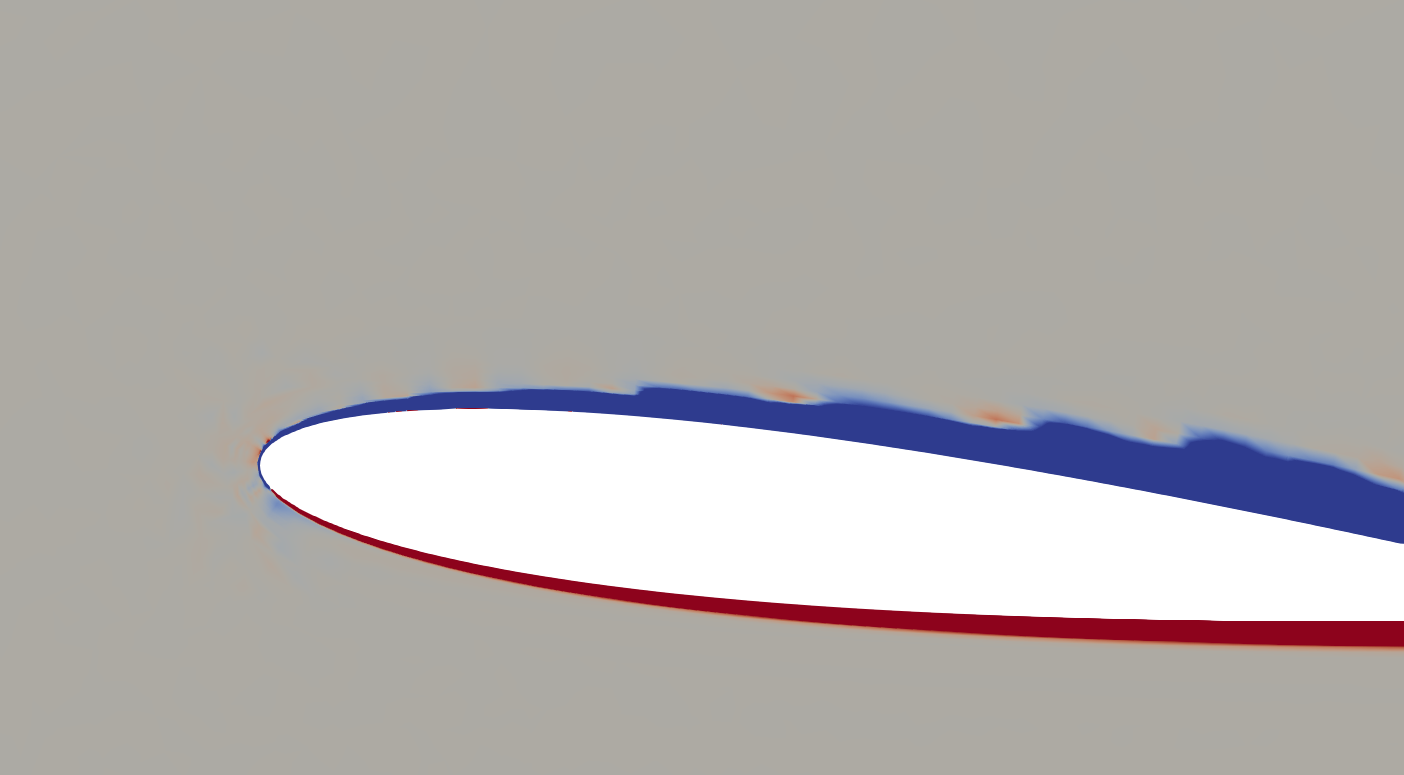
\includegraphics[width=1\textwidth]{figures/zonal_adapt_results/vorticity_plots/v2/M0/spavg/phase_150.png}
			\caption{M0\_nz25 mesh, $\psi$ = $150^\circ$}
			\label{fig:M0_sp_psi150}
		\end{subfigure}
	\end{center}
	\begin{subfigure}[b]{0.475\textwidth}
		\centering
		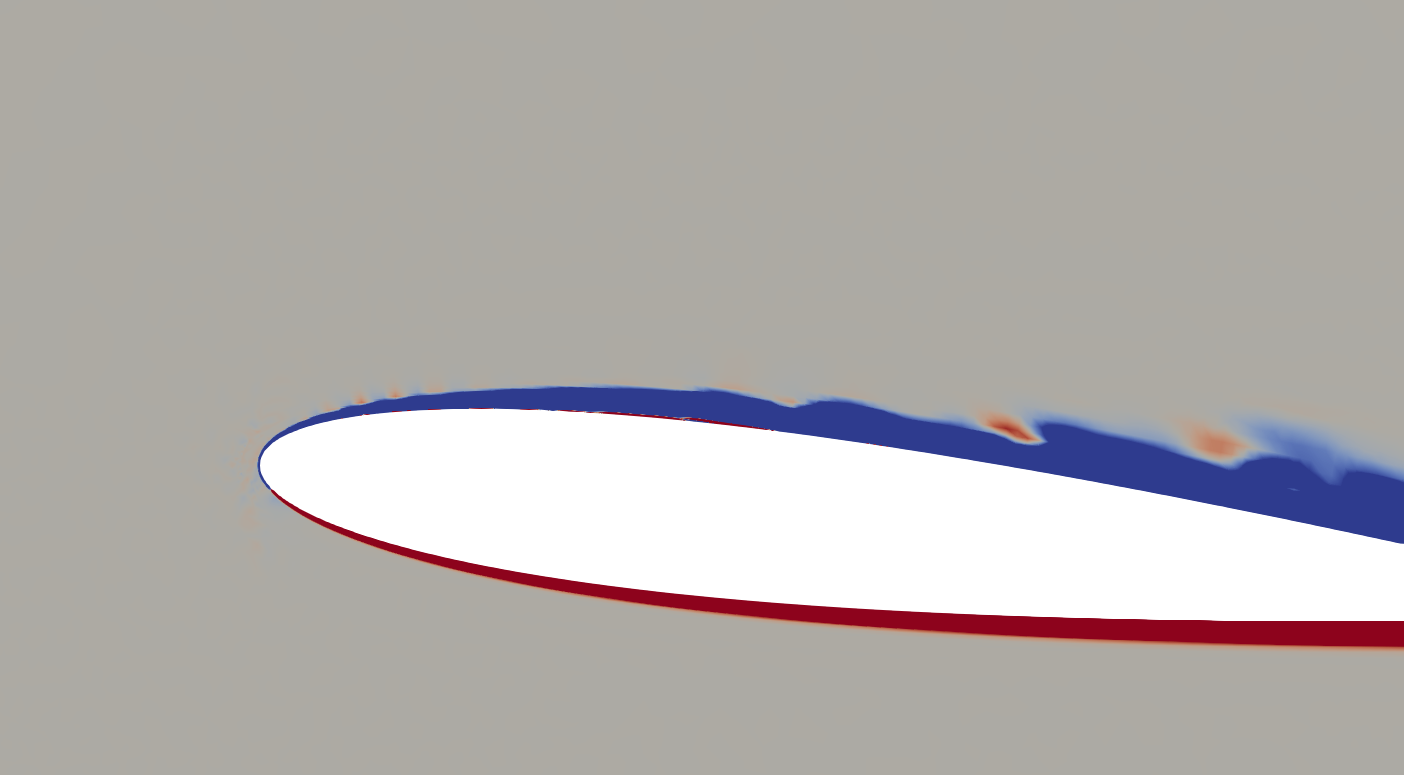
\includegraphics[width=1\textwidth]{figures/zonal_adapt_results/vorticity_plots/v2/Mza1_25/spavg/phase_150.png}
		\caption{Mza1\_nz25 mesh, $\psi$ = $150^\circ$}
		\label{fig:Mza1_25_sp_psi150}
	\end{subfigure}
	\begin{subfigure}[b]{0.475\textwidth}
		\centering
		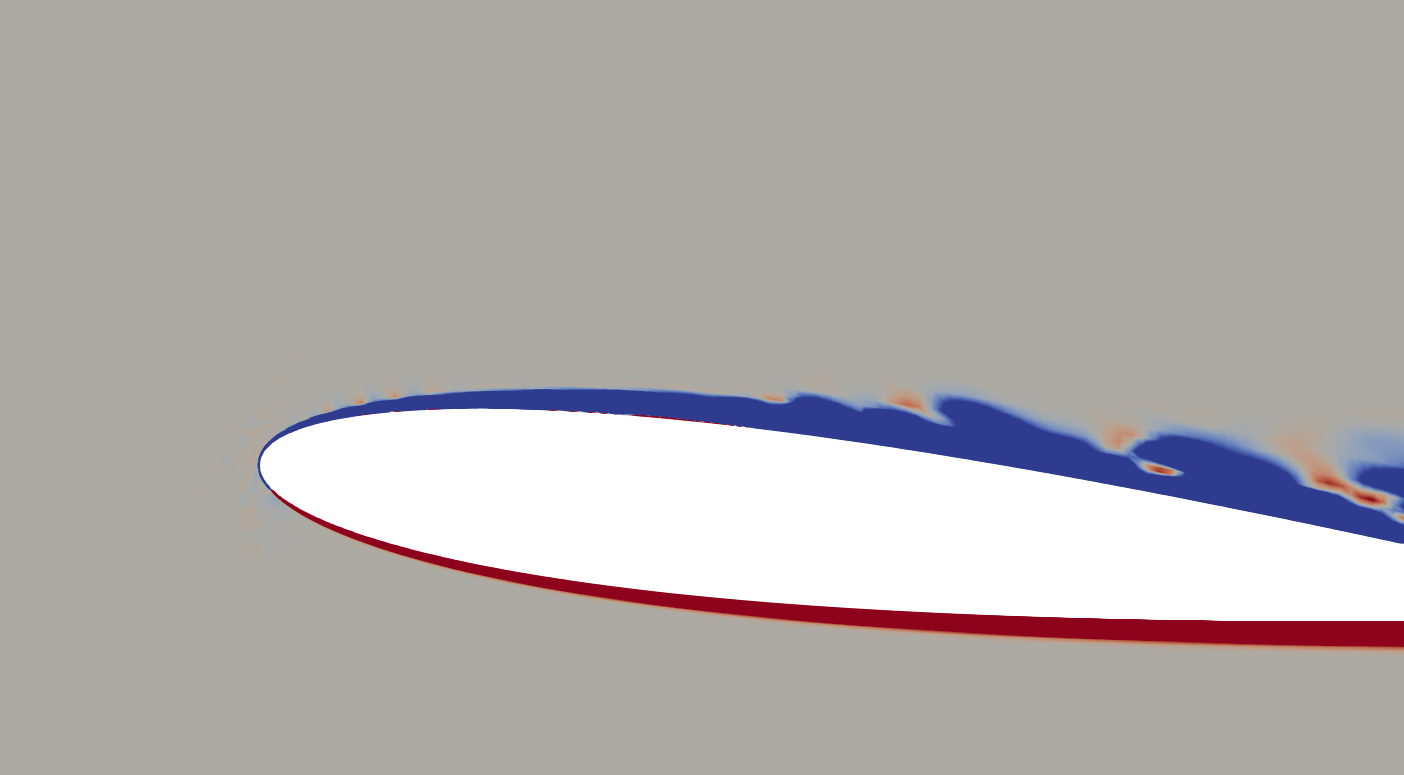
\includegraphics[width=1\textwidth]{figures/zonal_adapt_results/vorticity_plots/v2/Mza1_50/spavg/phase_150.png}
		\caption{Mza1\_nz50 mesh, $\psi$ = $150^\circ$}
		\label{fig:Mza1_50_sp_psi150}
	\end{subfigure}
	%	\begin{subfigure}[b]{0.475\textwidth}
	%		\centering
	%		\includegraphics[width=1\textwidth]{figures/zonal_adapt_results/vorticity_plots/v2/Mza1_100/spavg/phase_150.png}
	%		\caption{Mza1\_100 mesh, $\psi$ = $150^\circ$}
	%		\label{fig:Mza1_100_sp_psi150}
	%	\end{subfigure}
	%	\begin{subfigure}[b]{0.475\textwidth}
	%	\centering
	%	\includegraphics[width=1\textwidth]{figures/zonal_adapt_results/vorticity_plots/v2/Mza2_25/spavg/phase_150.png}
	%	\caption{Mza2\_25 mesh, $\psi$ = $150^\circ$}
	%	\label{fig:Mza2_25_sp_psi150}
	%	\end{subfigure}
	\begin{subfigure}[b]{0.475\textwidth}
		\centering
		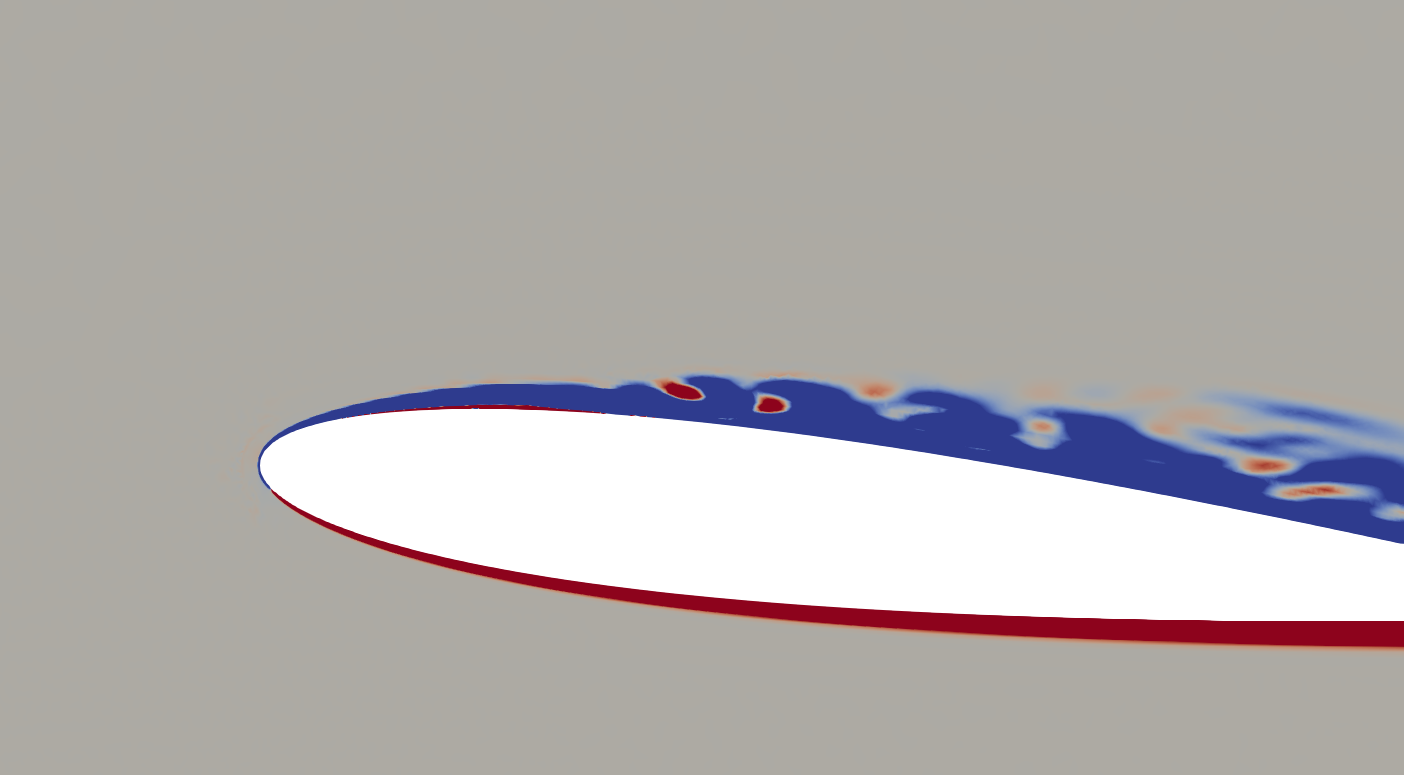
\includegraphics[width=1\textwidth]{figures/zonal_adapt_results/vorticity_plots/v2/Mza2_50/spavg/phase_150.png}
		\caption{Mza2\_nz50 mesh, $\psi$ = $150^\circ$}
		\label{fig:Mza2_50_sp_psi150}
	\end{subfigure}	
	\begin{subfigure}[b]{0.475\textwidth}
		\centering
		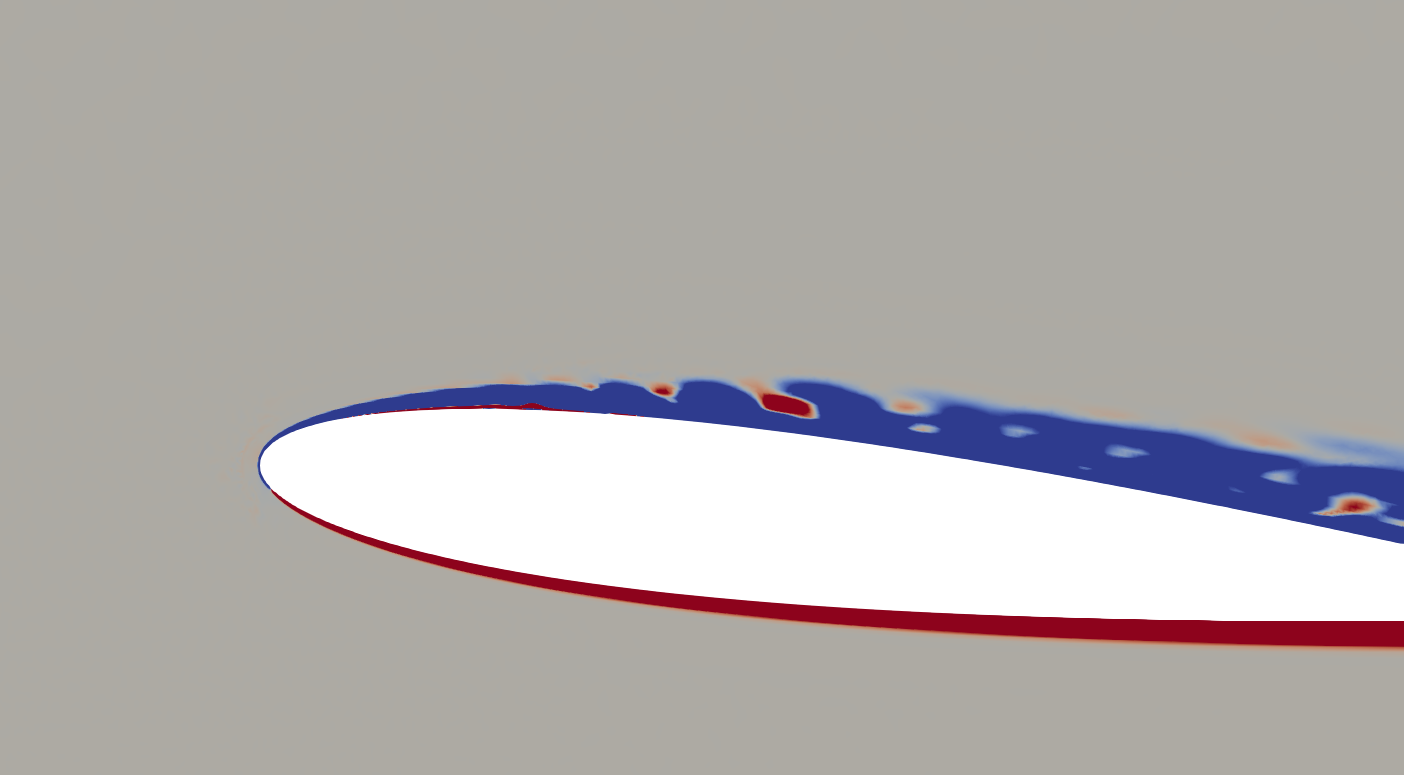
\includegraphics[width=1\textwidth]{figures/zonal_adapt_results/vorticity_plots/v2/Mza2_100/spavg/phase_150.png}
		\caption{Mza2\_nz100 mesh, $\psi$ = $150^\circ$}
		\label{fig:Mza2_100_sp_psi150}
	\end{subfigure}
	\begin{subfigure}[b]{0.475\textwidth}
		\centering
		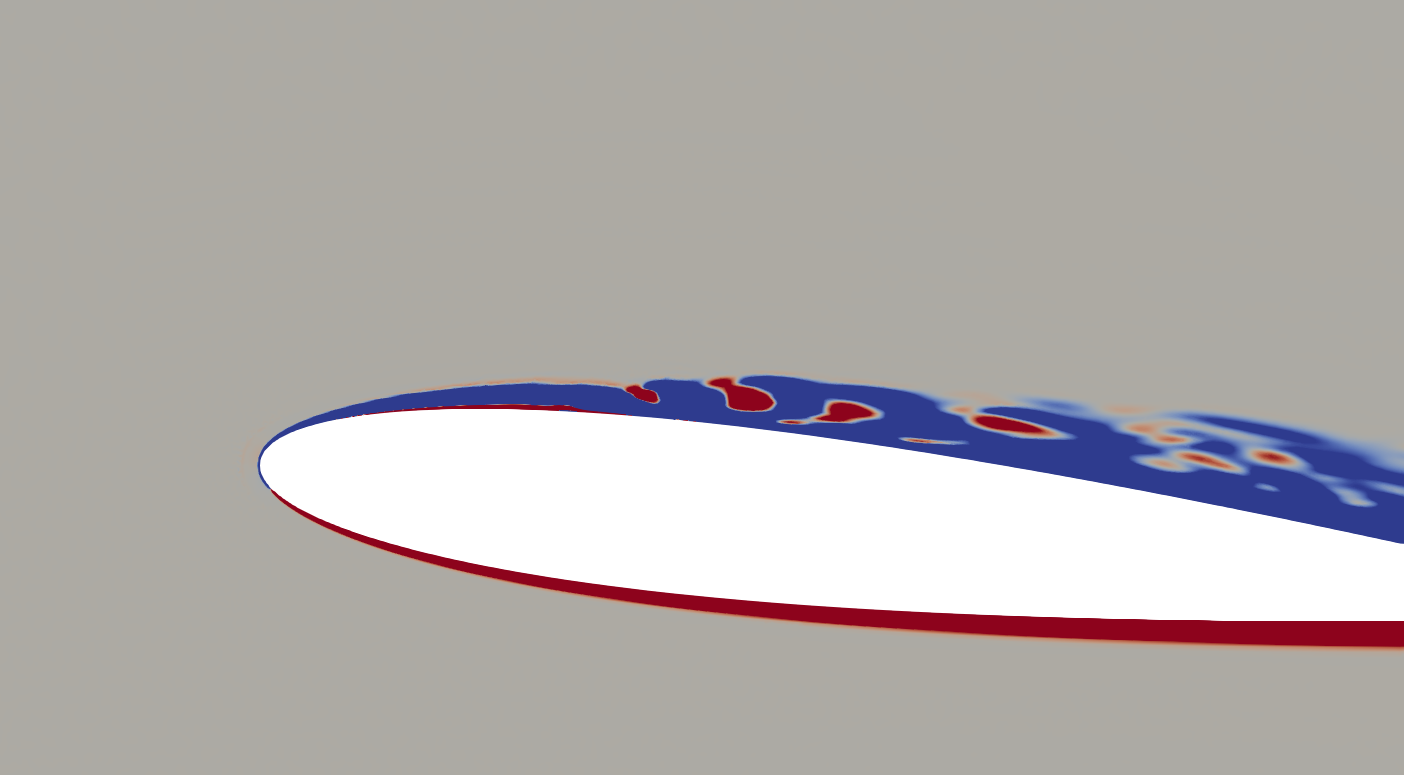
\includegraphics[width=1\textwidth]{figures/zonal_adapt_results/vorticity_plots/v2/Mza3_50/spavg/phase_150.png}
		\caption{Mza3\_nz50 mesh, $\psi$ = $150^\circ$}
		\label{fig:Mza3_50_sp_psi150}
	\end{subfigure}
	\begin{subfigure}[b]{0.475\textwidth}
		\centering
		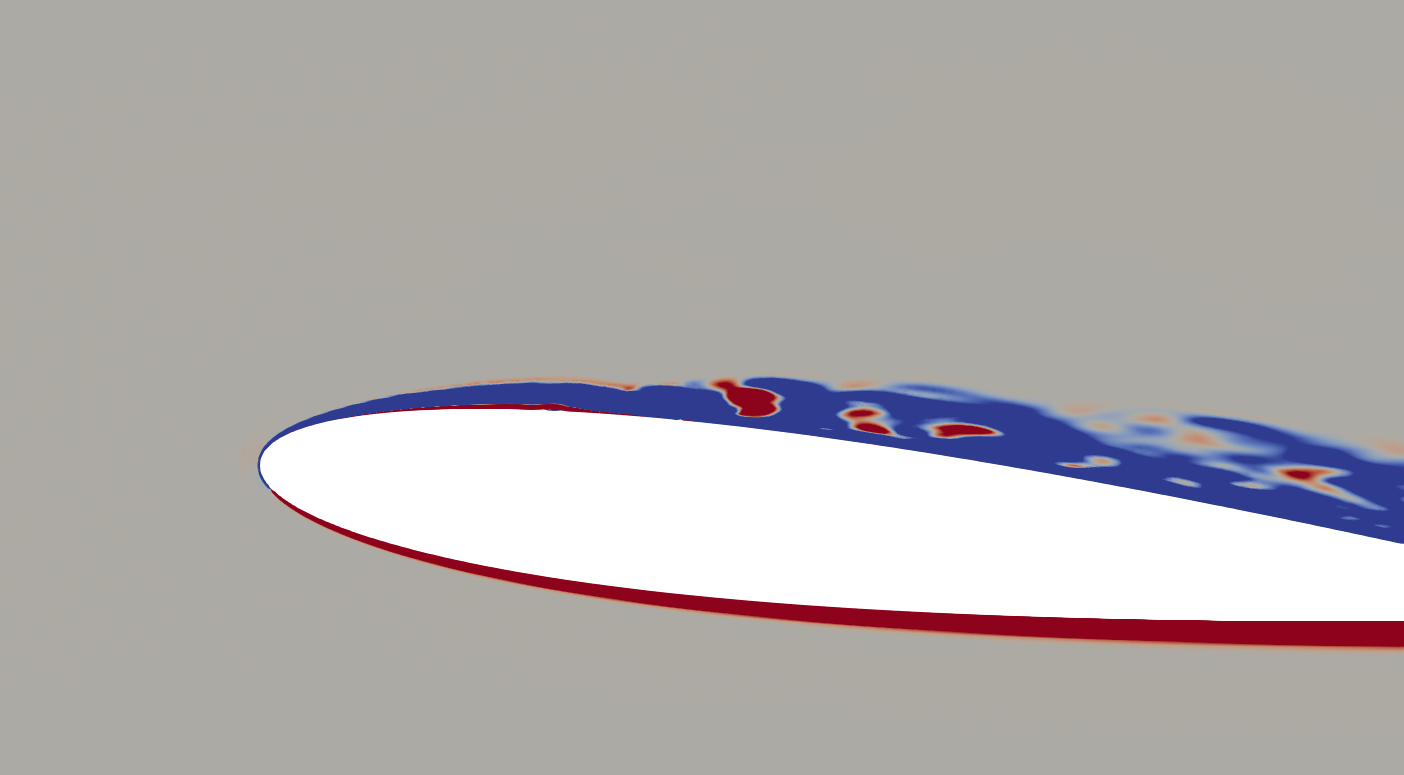
\includegraphics[width=1\textwidth]{figures/zonal_adapt_results/vorticity_plots/v2/Mza3_100/spavg/phase_150.png}
		\caption{Mza3\_nz100 mesh, $\psi$ = $150^\circ$}
		\label{fig:Mza3_100_sp_psi150}
	\end{subfigure}
	\caption{Adaptive LES at $Re=40,000$: spanwise vorticity at $\psi$ = $150^\circ$}
	\label{fig:vorticity_zonal_150}
\end{figure}




%%=====================================
%% Phase = 180
%%=====================================


\begin{figure}[H]
	\centering
	\begin{center}
	\begin{subfigure}[b]{0.475\textwidth}
		\centering
		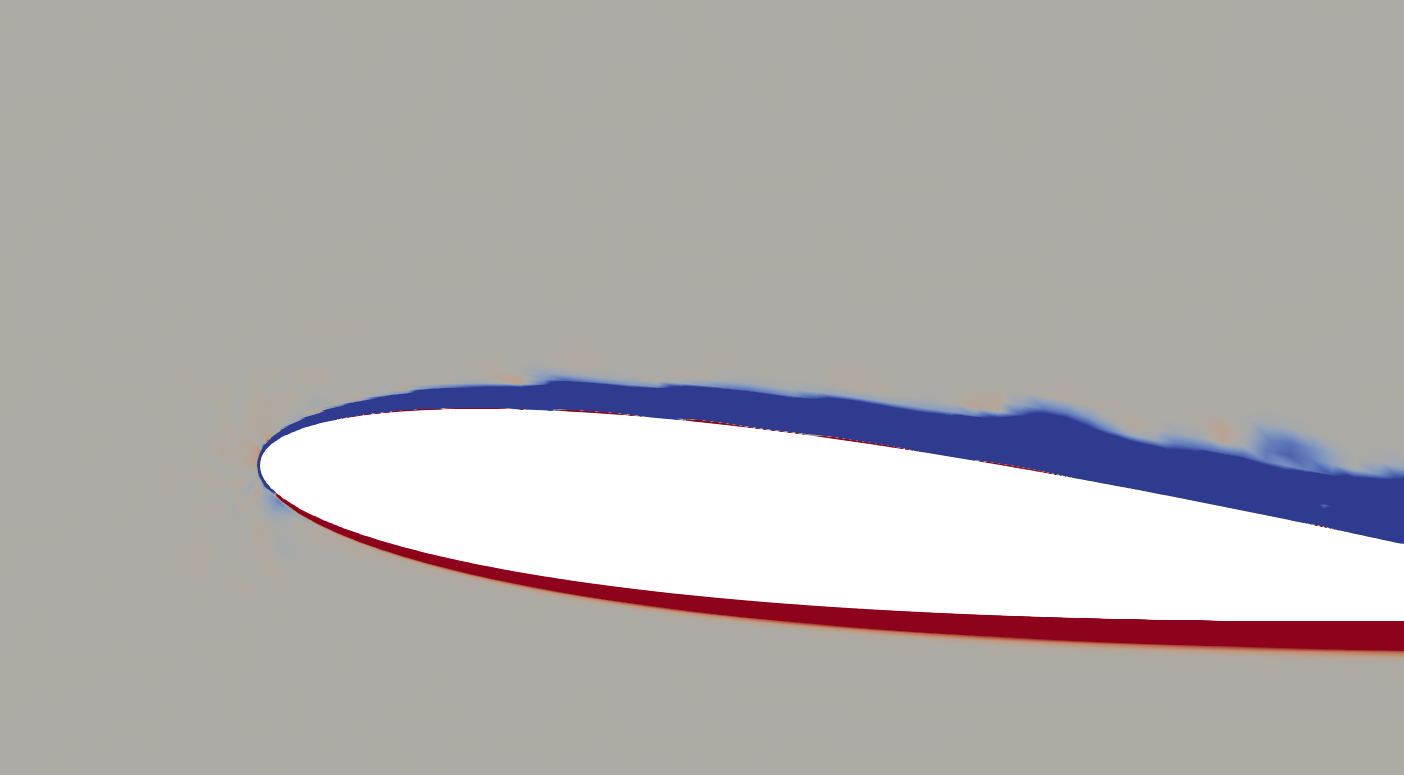
\includegraphics[width=1\textwidth]{figures/zonal_adapt_results/vorticity_plots/v2/M0/spavg/phase_180.png}
		\caption{M0\_nz25 mesh, $\psi$ = $180^\circ$}
		\label{fig:M0_sp_psi180}
	\end{subfigure}
	\end{center}
	\begin{subfigure}[b]{0.475\textwidth}
	\centering
	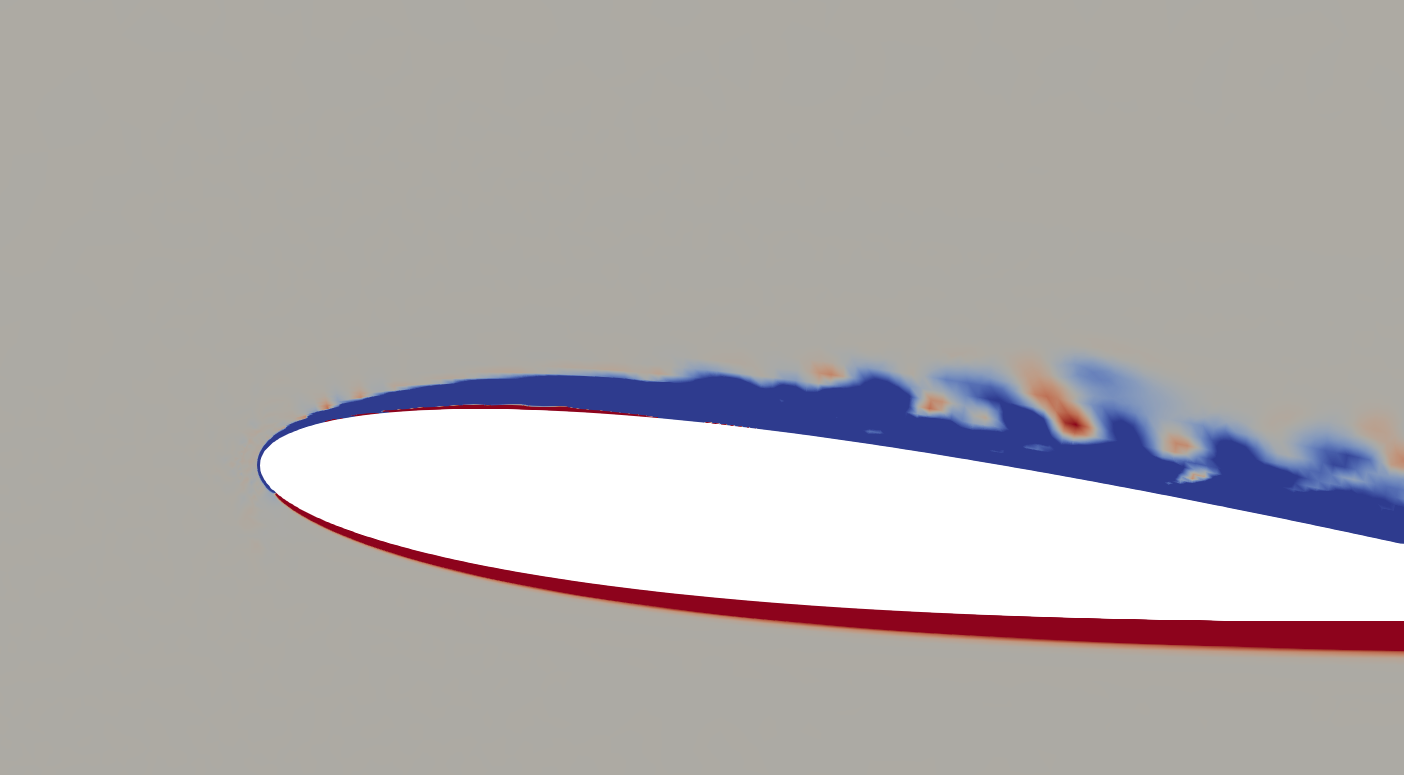
\includegraphics[width=1\textwidth]{figures/zonal_adapt_results/vorticity_plots/v2/Mza1_25/spavg/phase_180.png}
	\caption{Mza1\_nz25 mesh, $\psi$ = $180^\circ$}
	\label{fig:Mza1_25_sp_psi180}
\end{subfigure}
	\begin{subfigure}[b]{0.475\textwidth}
		\centering
		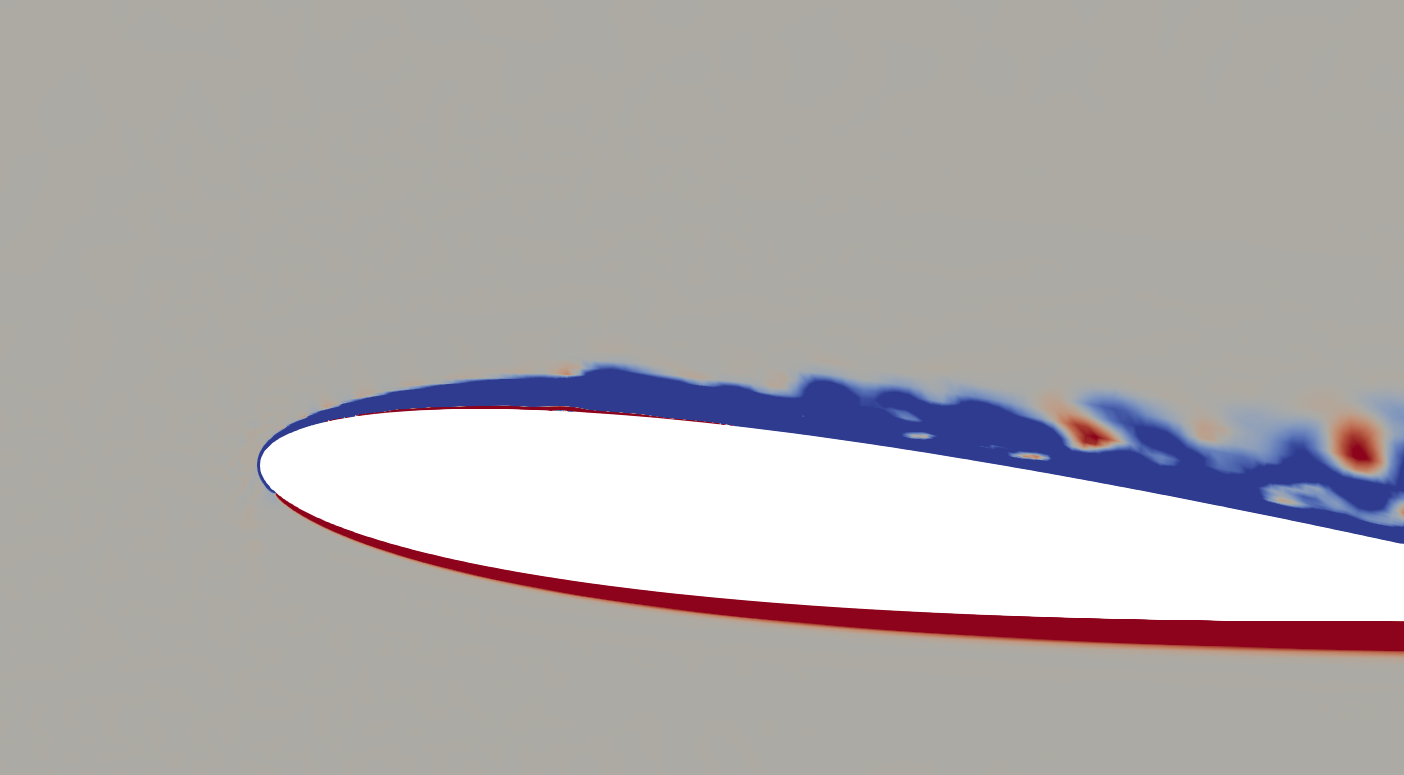
\includegraphics[width=1\textwidth]{figures/zonal_adapt_results/vorticity_plots/v2/Mza1_50/spavg/phase_180.png}
		\caption{Mza1\_nz50 mesh, $\psi$ = $180^\circ$}
		\label{fig:Mza1_50_sp_psi180}
	\end{subfigure}
%	\begin{subfigure}[b]{0.475\textwidth}
%		\centering
%		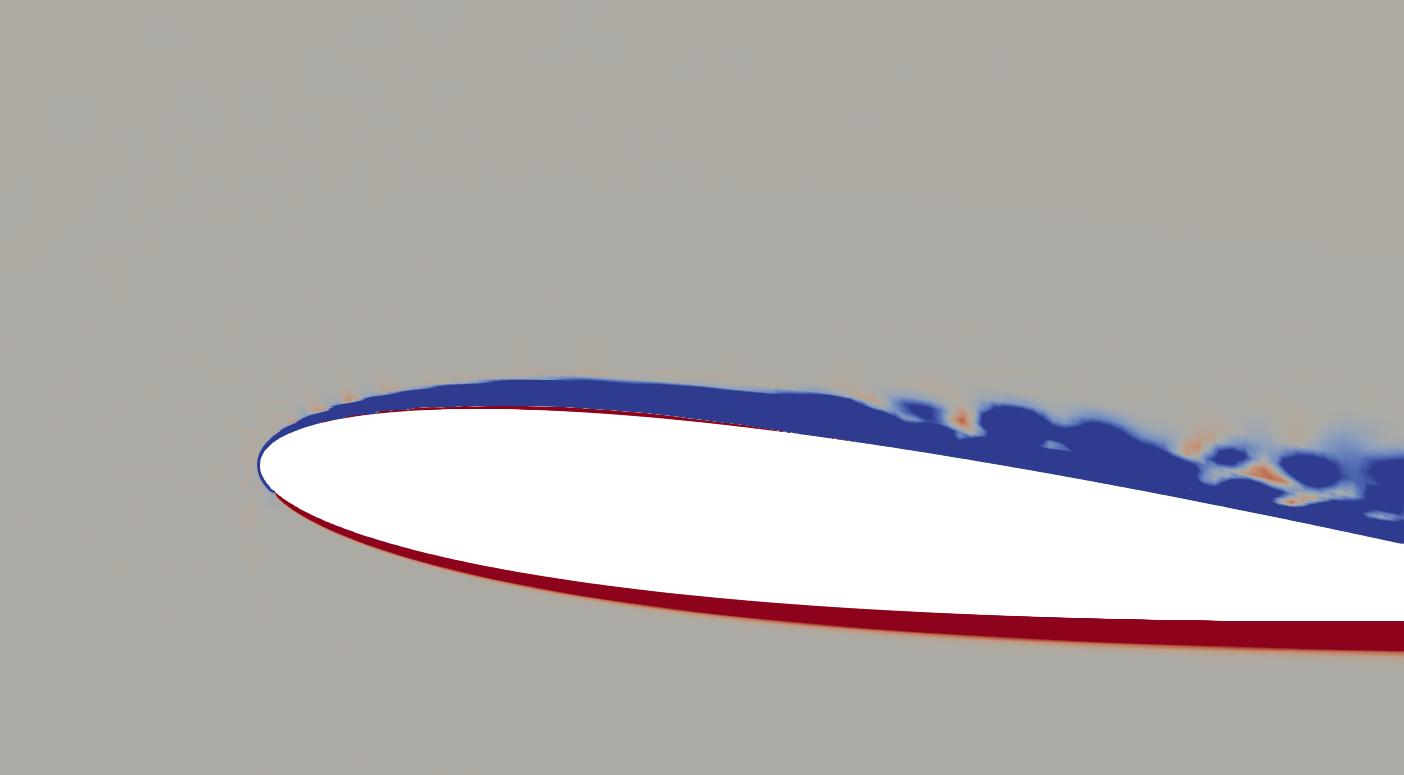
\includegraphics[width=1\textwidth]{figures/zonal_adapt_results/vorticity_plots/v2/Mza1_100/spavg/phase_180.png}
%		\caption{Mza1\_100 mesh, $\psi$ = $180^\circ$}
%		\label{fig:Mza1_100_sp_psi180}
%	\end{subfigure}
%	\begin{subfigure}[b]{0.475\textwidth}
%	\centering
%	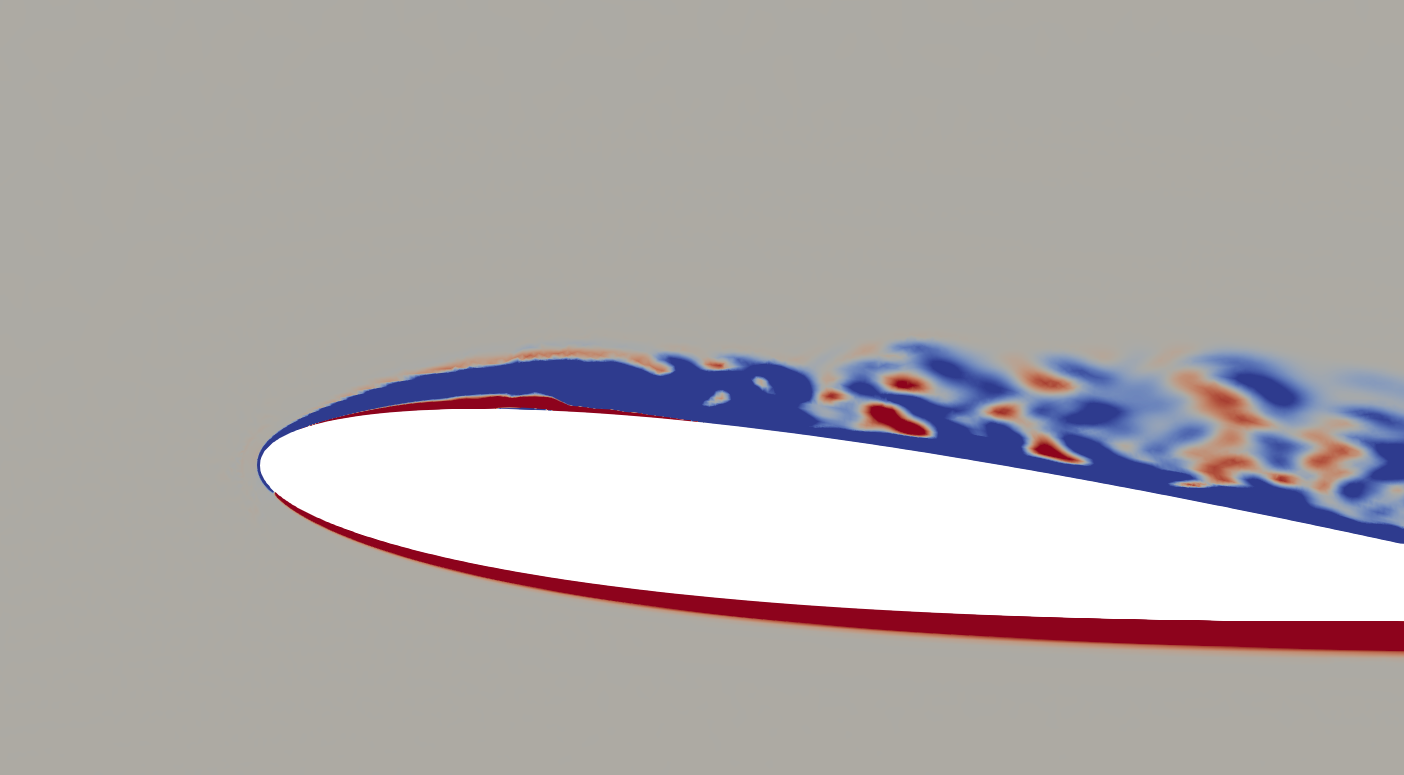
\includegraphics[width=1\textwidth]{figures/zonal_adapt_results/vorticity_plots/v2/Mza2_25/spavg/phase_180.png}
%	\caption{Mza2\_25 mesh, $\psi$ = $180^\circ$}
%	\label{fig:Mza2_25_sp_psi180}
%	\end{subfigure}
	\begin{subfigure}[b]{0.475\textwidth}
		\centering
		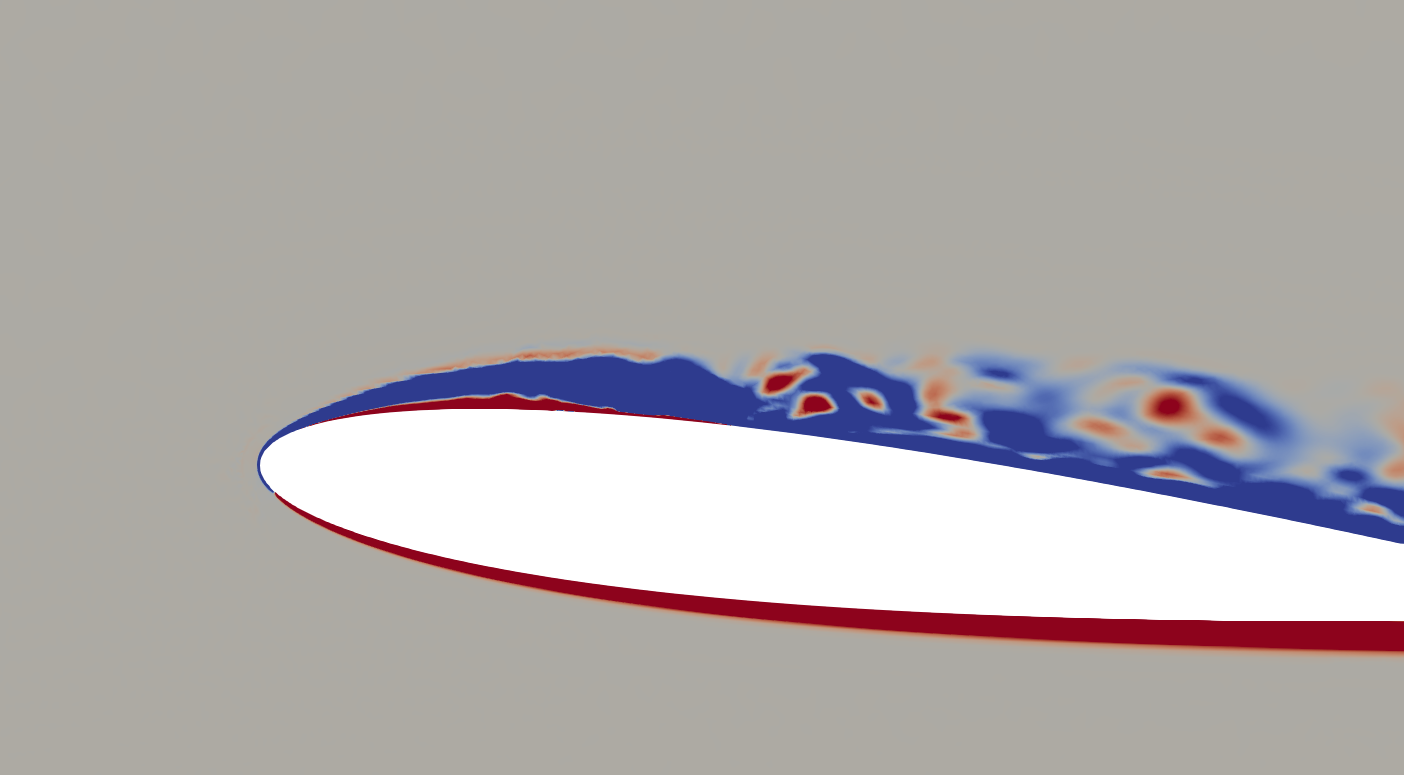
\includegraphics[width=1\textwidth]{figures/zonal_adapt_results/vorticity_plots/v2/Mza2_50/spavg/phase_180.png}
		\caption{Mza2\_nz50 mesh, $\psi$ = $180^\circ$}
		\label{fig:Mza2_50_sp_psi180}
	\end{subfigure}	
	\begin{subfigure}[b]{0.475\textwidth}
		\centering
		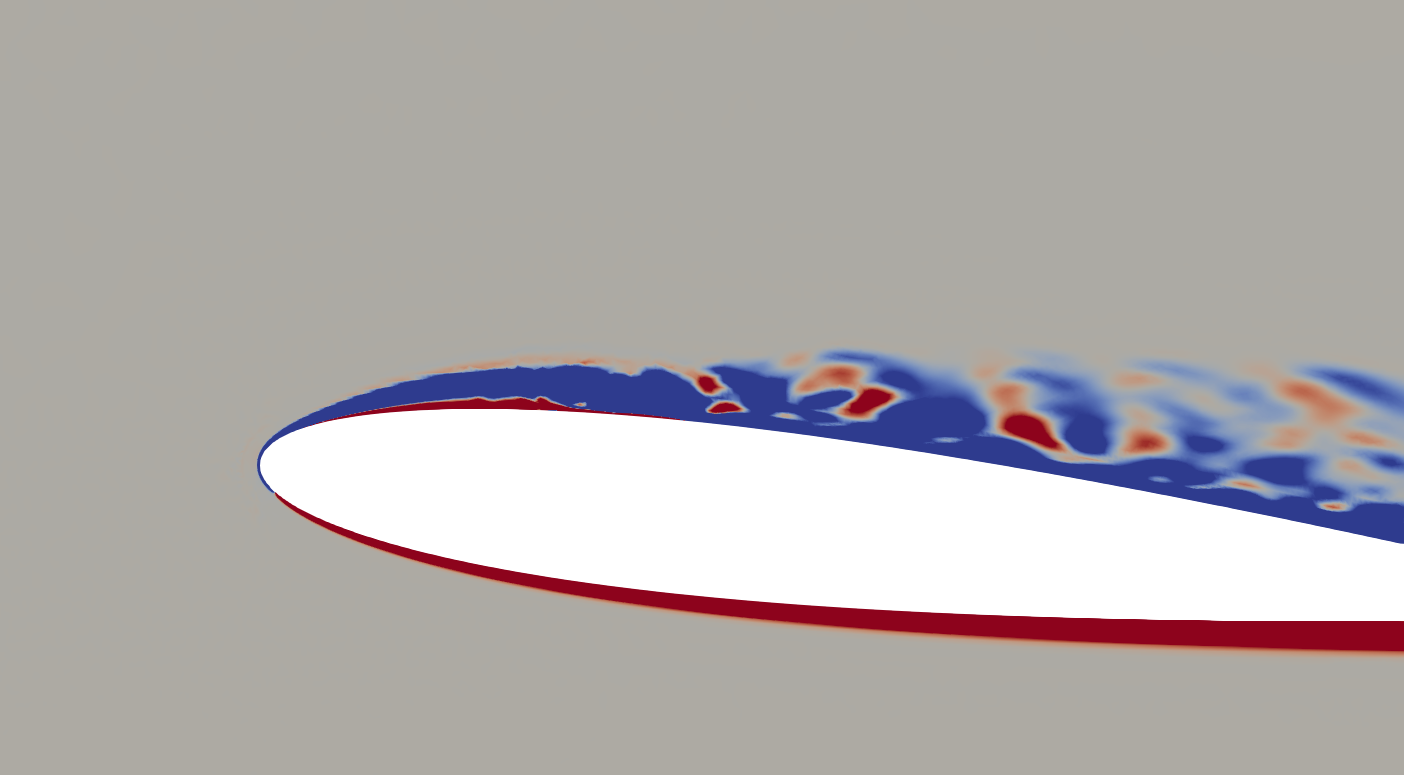
\includegraphics[width=1\textwidth]{figures/zonal_adapt_results/vorticity_plots/v2/Mza2_100/spavg/phase_180.png}
		\caption{Mza2\_nz100 mesh, $\psi$ = $180^\circ$}
		\label{fig:Mza2_100_sp_psi180}
	\end{subfigure}
	\begin{subfigure}[b]{0.475\textwidth}
	\centering
	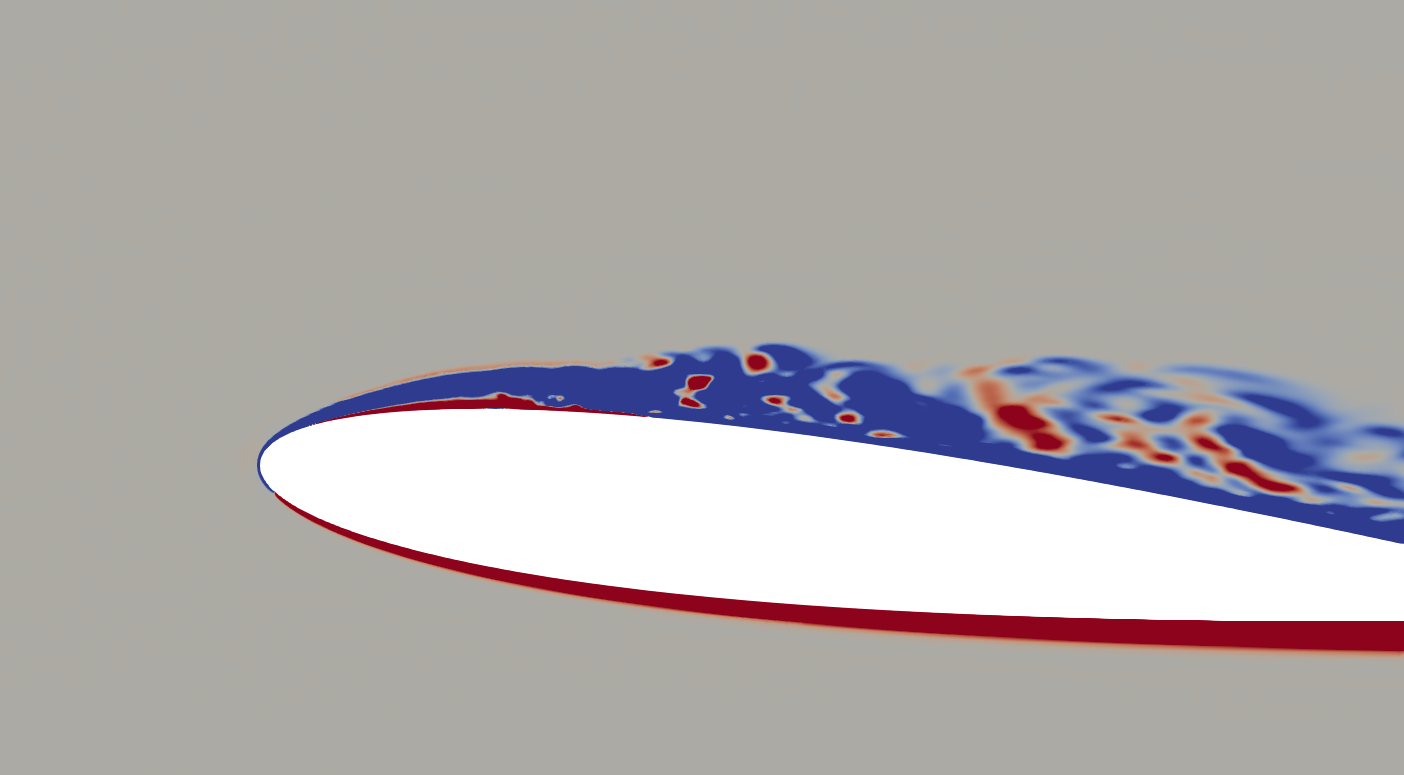
\includegraphics[width=1\textwidth]{figures/zonal_adapt_results/vorticity_plots/v2/Mza3_50/spavg/phase_180.png}
	\caption{Mza3\_nz50 mesh, $\psi$ = $180^\circ$}
	\label{fig:Mza3_50_sp_psi180}
	\end{subfigure}
	\begin{subfigure}[b]{0.475\textwidth}
		\centering
		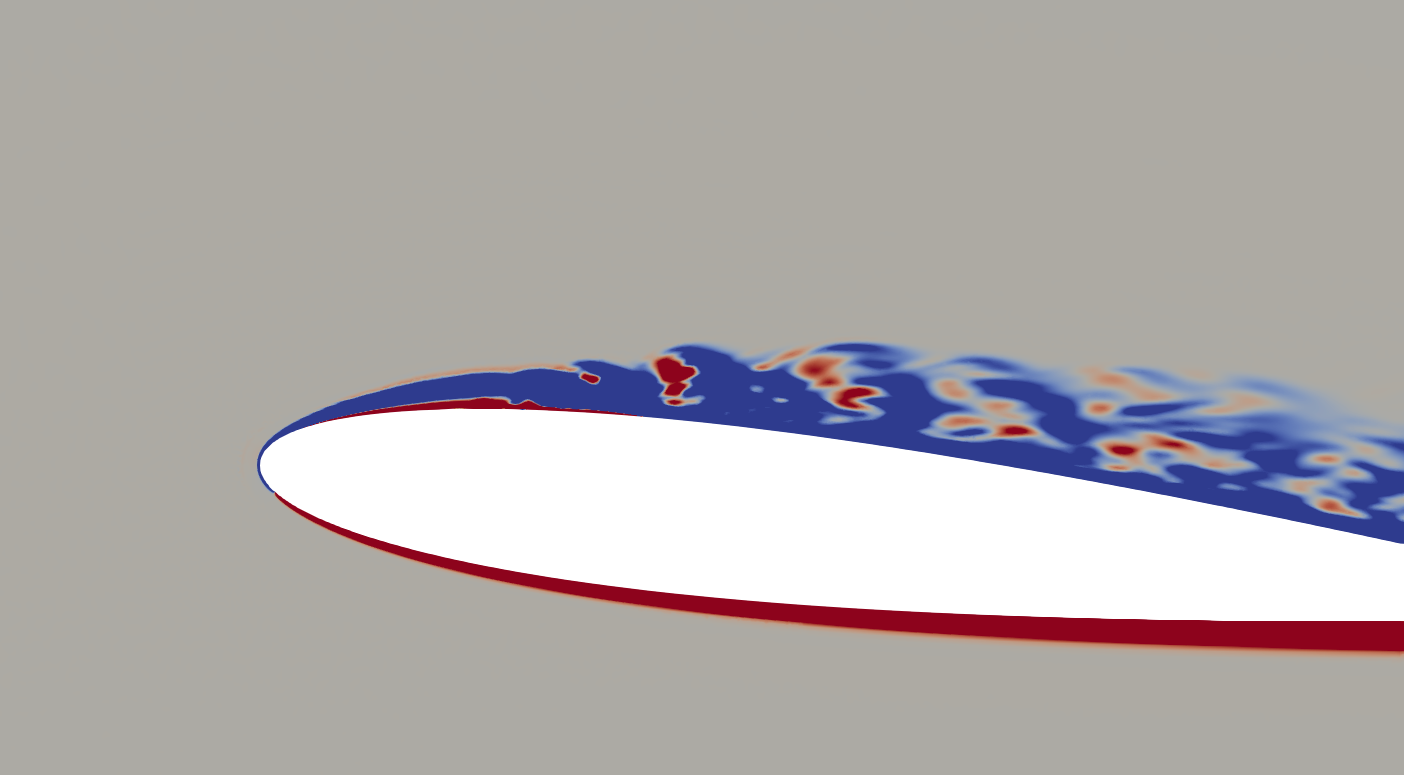
\includegraphics[width=1\textwidth]{figures/zonal_adapt_results/vorticity_plots/v2/Mza3_100/spavg/phase_180.png}
		\caption{Mza3\_nz100 mesh, $\psi$ = $180^\circ$}
		\label{fig:Mza3_100_sp_psi180}
	\end{subfigure}
	\caption{Spanwise vorticity comparison at $\psi$ = $180^\circ$ for different meshes}
	\label{fig:vorticity_zonal_180}
\end{figure}

%%=====================================
%% Phase = 210
%%=====================================


\begin{figure}[H]
	\centering
	\begin{center}
		\begin{subfigure}[b]{0.475\textwidth}
		\centering
		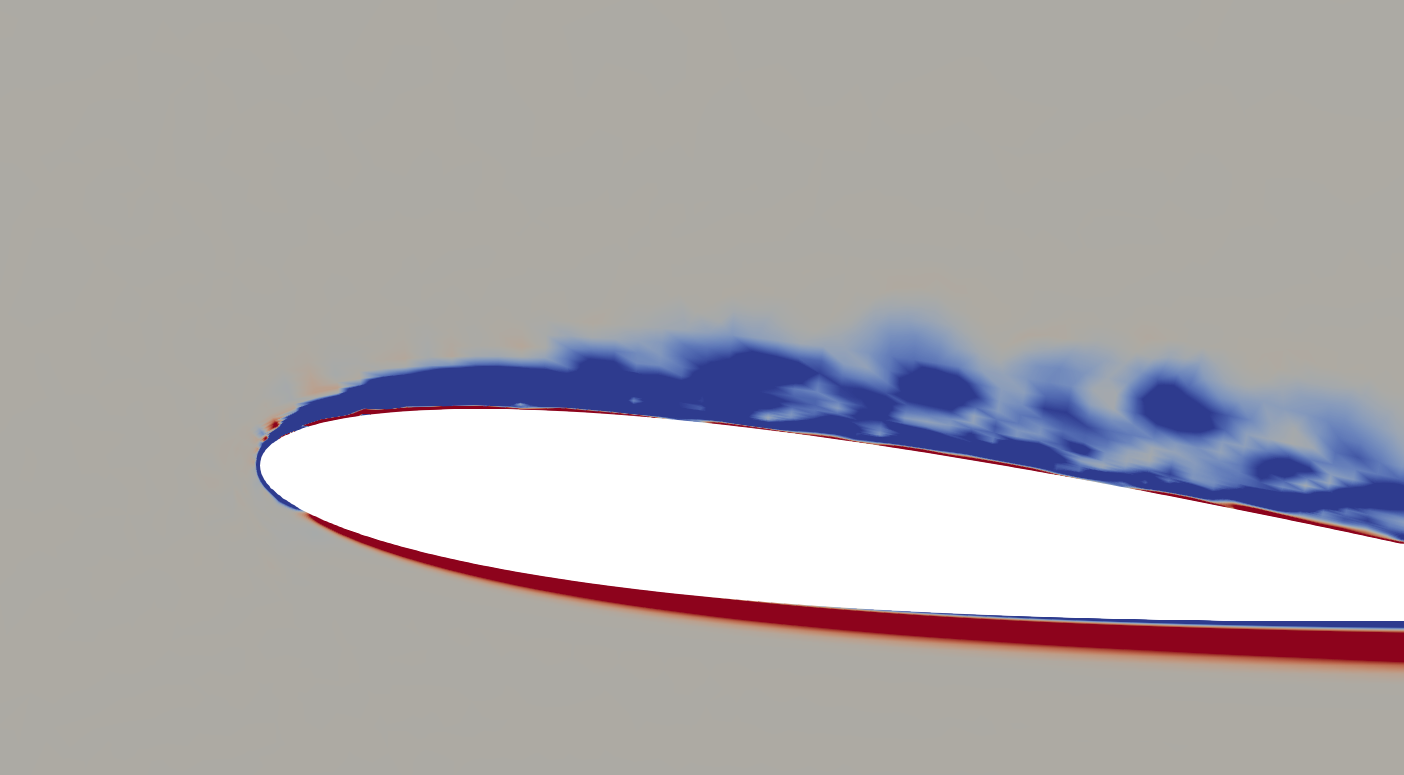
\includegraphics[width=1\textwidth]{figures/zonal_adapt_results/vorticity_plots/v2/M0/spavg/phase_210.png}
		\caption{M0\_nz25 mesh, $\psi$ = $210^\circ$}
		\label{fig:M0_sp_psi210}
		\end{subfigure}
	\end{center}
	\begin{subfigure}[b]{0.475\textwidth}
	\centering
	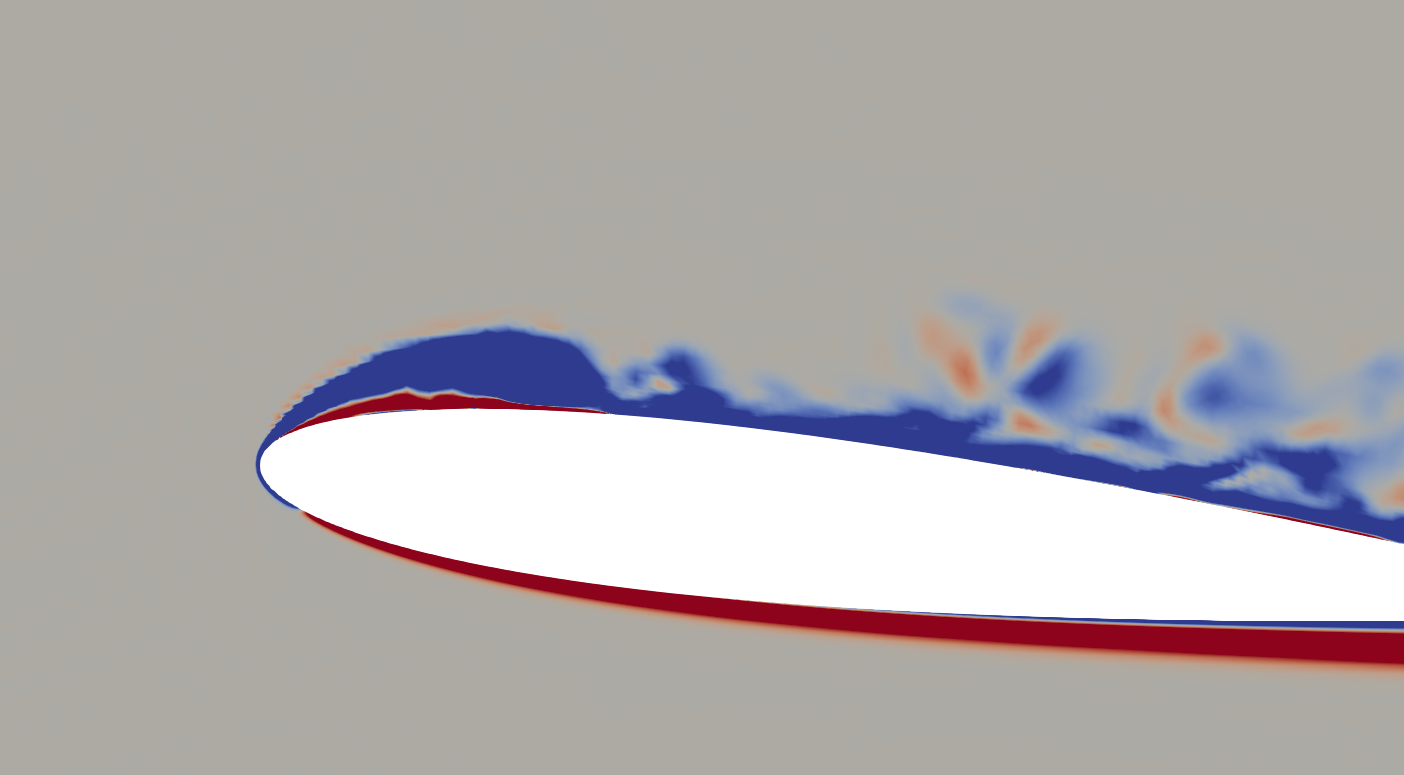
\includegraphics[width=1\textwidth]{figures/zonal_adapt_results/vorticity_plots/v2/Mza1_25/spavg/phase_210.png}
	\caption{Mza1\_nz25 mesh, $\psi$ = $210^\circ$}
	\label{fig:Mza1_25_sp_psi210}
	\end{subfigure}
	\begin{subfigure}[b]{0.475\textwidth}
		\centering
		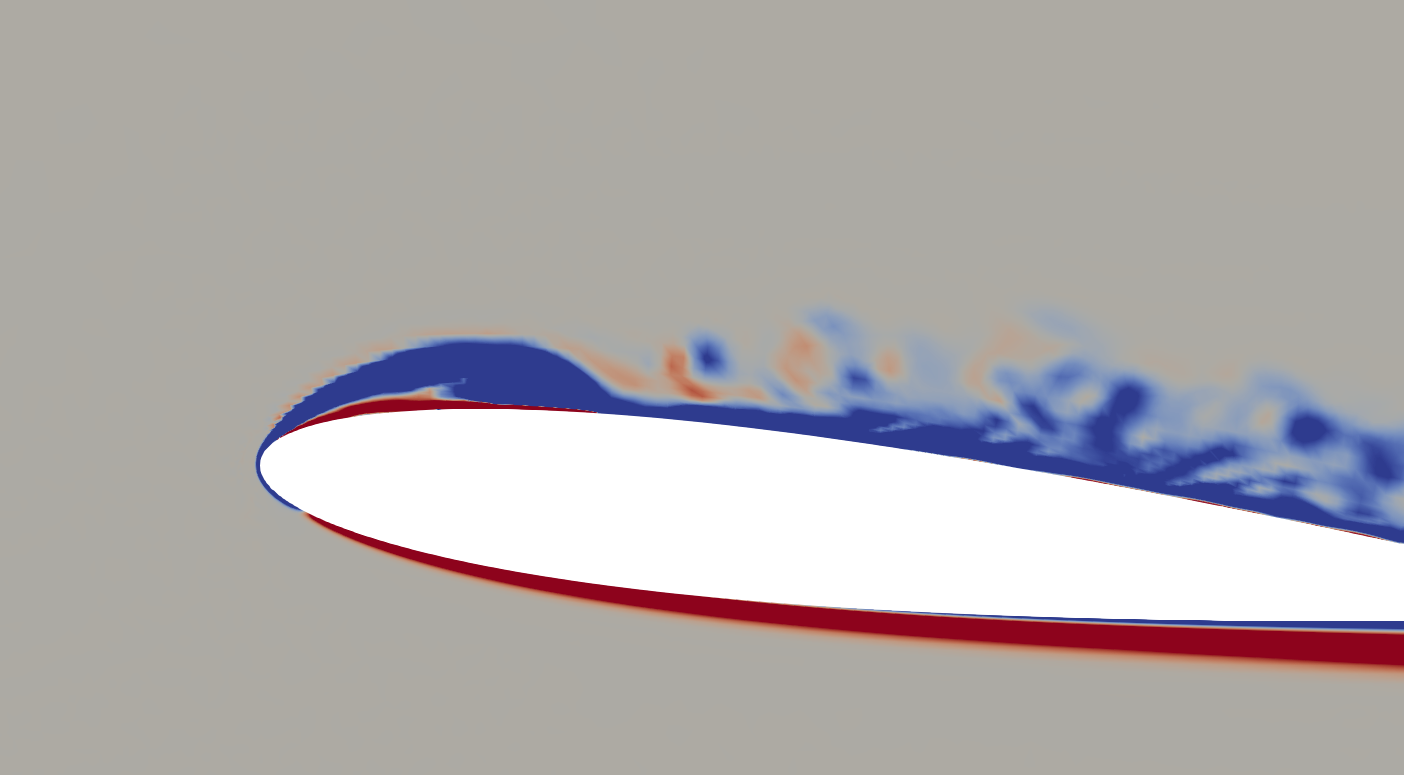
\includegraphics[width=1\textwidth]{figures/zonal_adapt_results/vorticity_plots/v2/Mza1_50/spavg/phase_210.png}
		\caption{Mza1\_nz50 mesh, $\psi$ = $210^\circ$}
		\label{fig:Mza1_50_sp_psi210}
	\end{subfigure}
%	\begin{subfigure}[b]{0.475\textwidth}
%		\centering
%		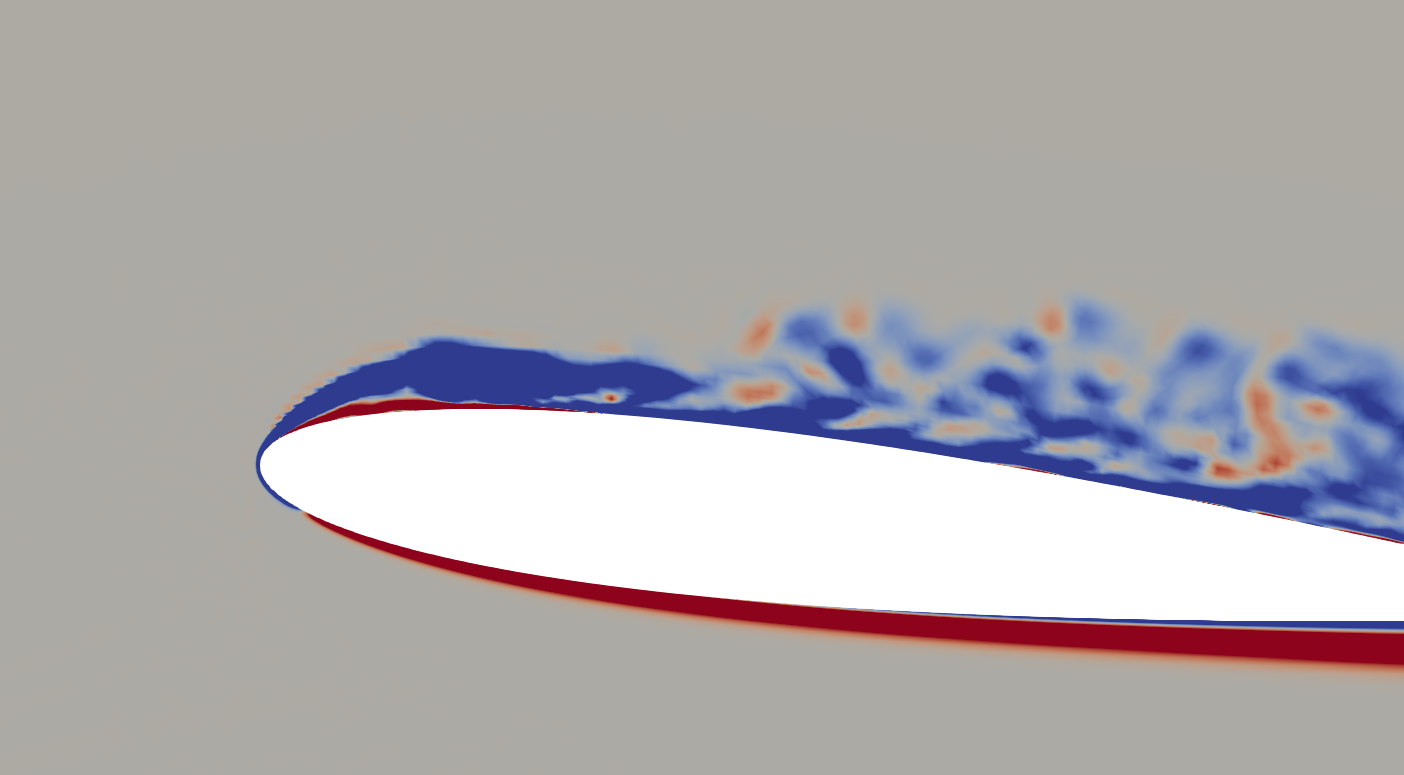
\includegraphics[width=1\textwidth]{figures/zonal_adapt_results/vorticity_plots/v2/Mza1_100/spavg/phase_210.png}
%		\caption{Mza1\_100 mesh, $\psi$ = $210^\circ$}
%		\label{fig:Mza1_100_sp_psi210}
%	\end{subfigure}
%	\begin{subfigure}[b]{0.475\textwidth}
%	\centering
%	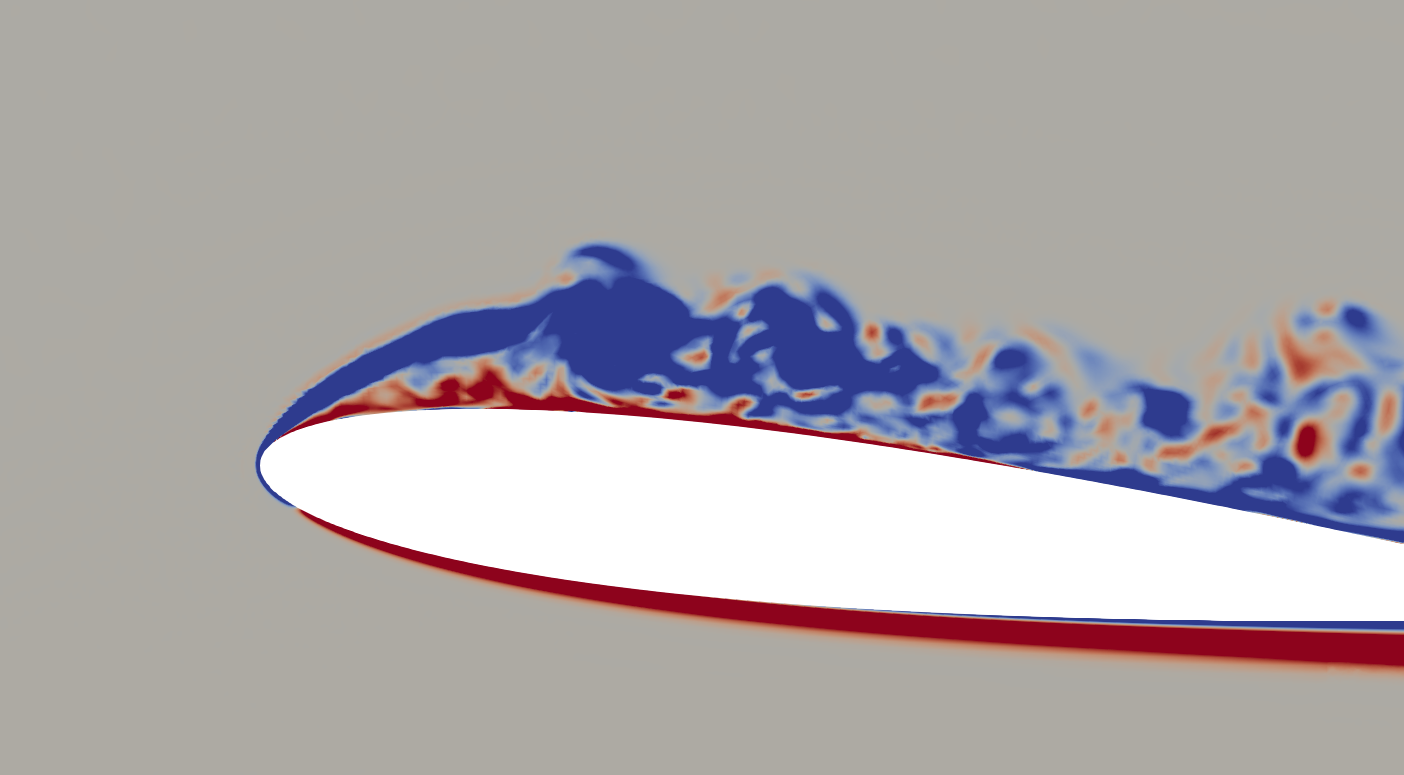
\includegraphics[width=1\textwidth]{figures/zonal_adapt_results/vorticity_plots/v2/Mza2_25/spavg/phase_210.png}
%	\caption{Mza2\_25 mesh, $\psi$ = $210^\circ$}
%	\label{fig:Mza2_25_sp_psi210}
%	\end{subfigure}	
	\begin{subfigure}[b]{0.475\textwidth}
		\centering
		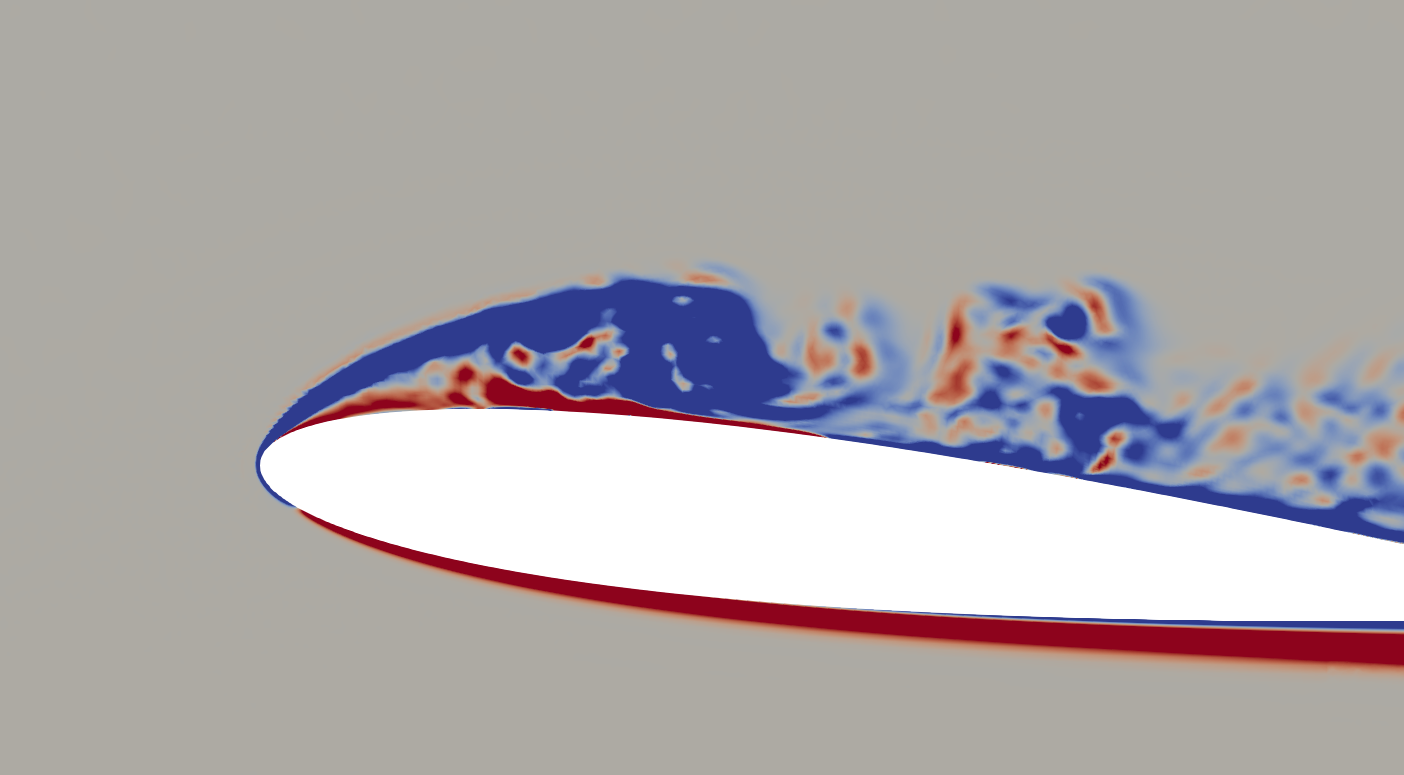
\includegraphics[width=1\textwidth]{figures/zonal_adapt_results/vorticity_plots/v2/Mza2_50/spavg/phase_210.png}
		\caption{Mza2\_nz50 mesh, $\psi$ = $210^\circ$}
		\label{fig:Mza2_50_sp_psi210}
	\end{subfigure}	
	\begin{subfigure}[b]{0.475\textwidth}
		\centering
		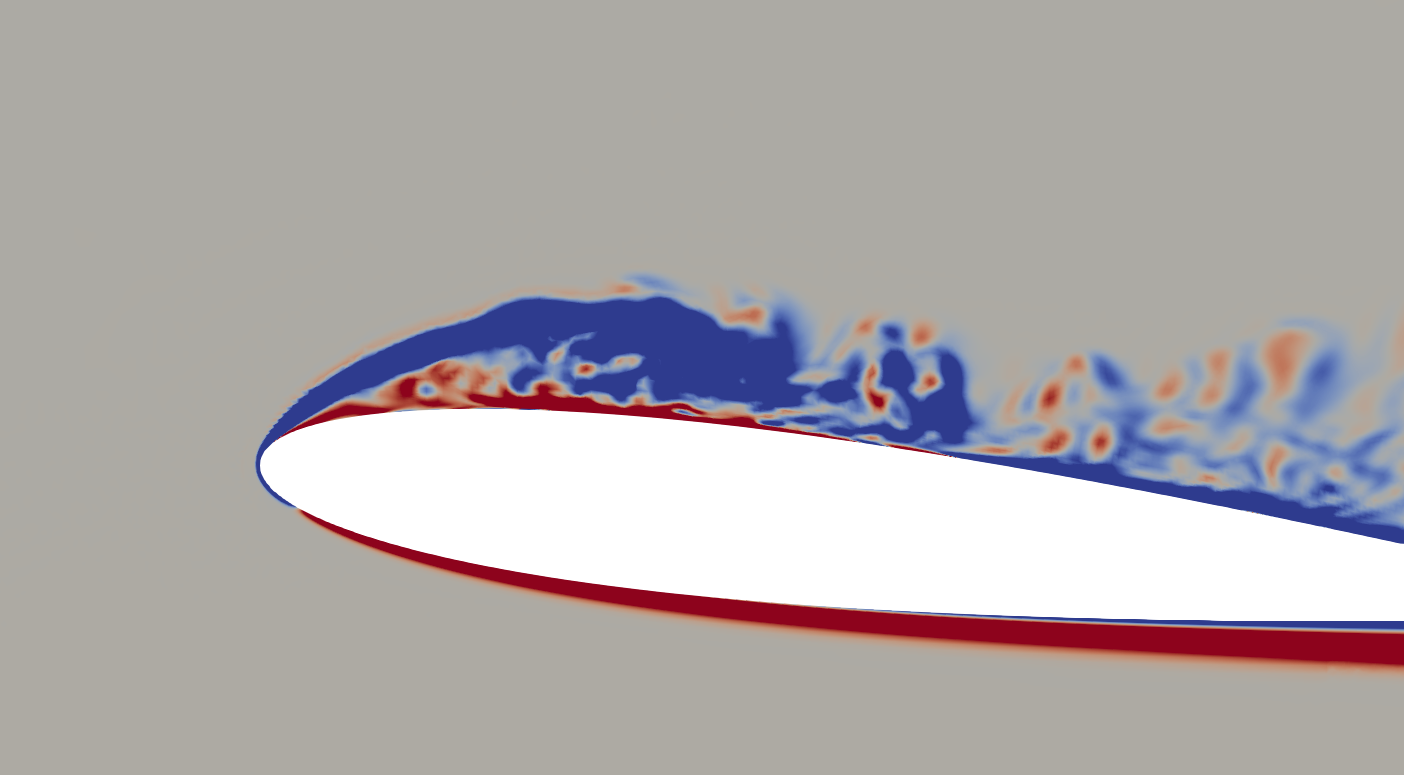
\includegraphics[width=1\textwidth]{figures/zonal_adapt_results/vorticity_plots/v2/Mza2_100/spavg/phase_210.png}
		\caption{Mza2\_nz100 mesh, $\psi$ = $210^\circ$}
		\label{fig:Mza2_100_sp_psi210}
	\end{subfigure}
	\begin{subfigure}[b]{0.475\textwidth}
	\centering
	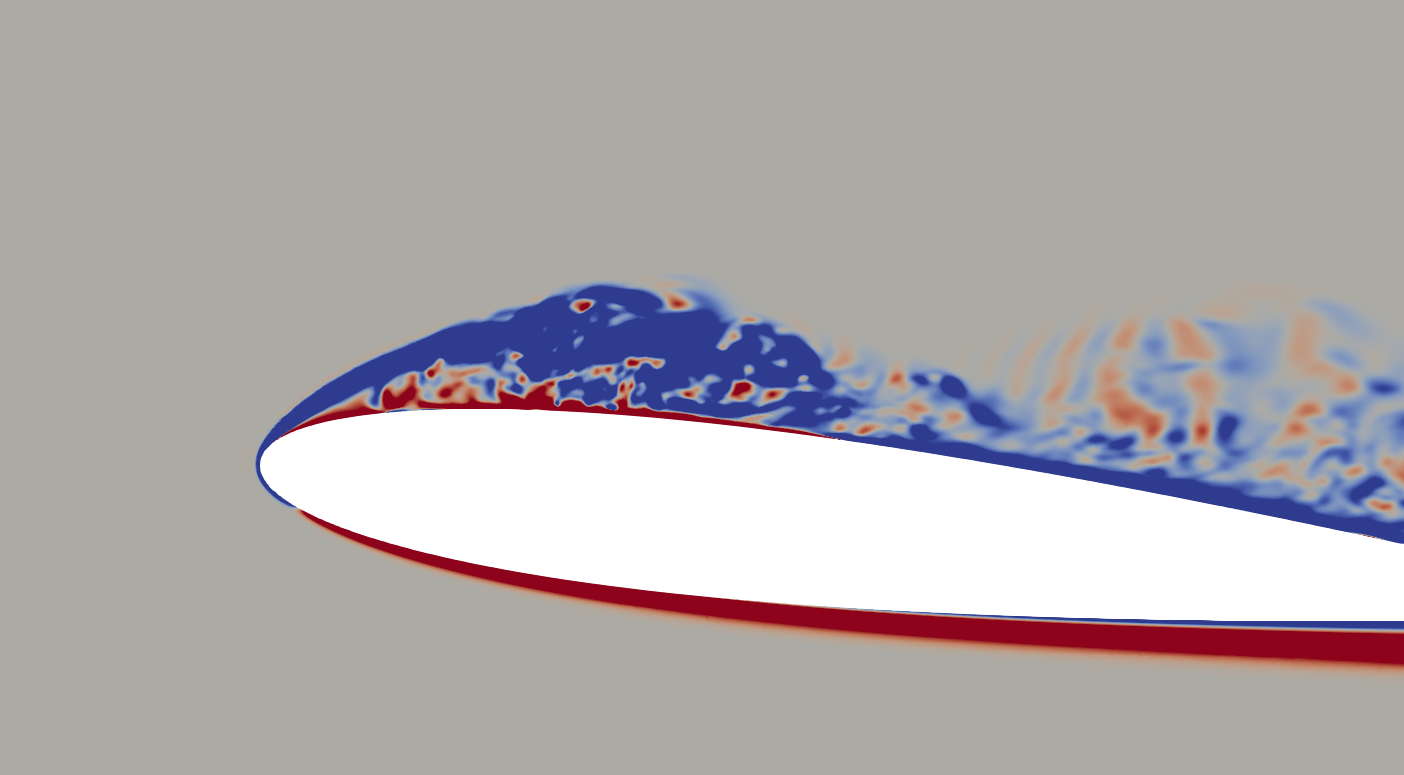
\includegraphics[width=1\textwidth]{figures/zonal_adapt_results/vorticity_plots/v2/Mza3_50/spavg/phase_210.png}
	\caption{Mza3\_nz50 mesh, $\psi$ = $210^\circ$}
	\label{fig:Mza3_50_sp_psi210}
\end{subfigure}
	\begin{subfigure}[b]{0.475\textwidth}
		\centering
		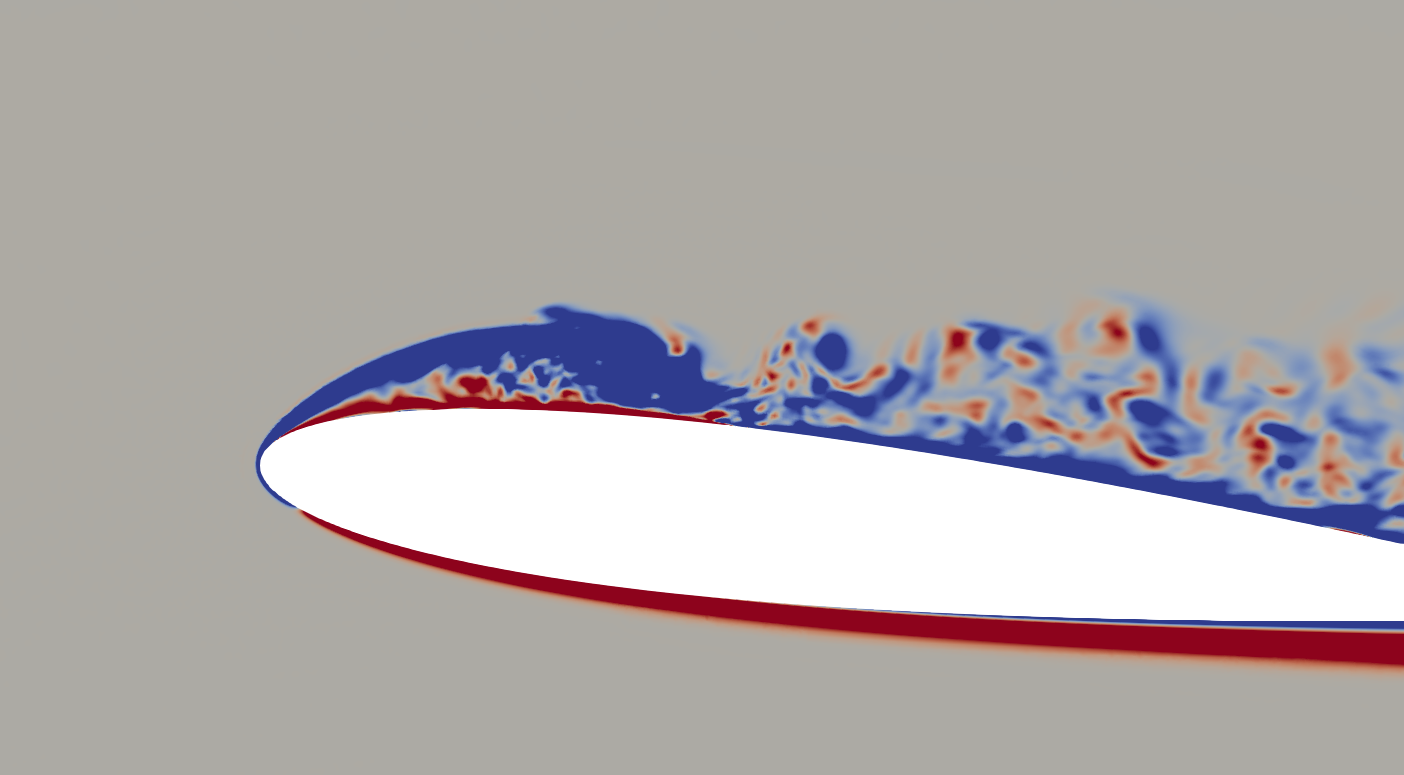
\includegraphics[width=1\textwidth]{figures/zonal_adapt_results/vorticity_plots/v2/Mza3_100/spavg/phase_210.png}
		\caption{Mza3\_nz100 mesh, $\psi$ = $210^\circ$}
		\label{fig:Mza3_100_sp_psi210}
	\end{subfigure}
	\caption{Spanwise vorticity comparison at $\psi$ = $210^\circ$ for different meshes}
	\label{fig:vorticity_zonal_210}
\end{figure}

%%=====================================
%% Phase = 240
%%=====================================


\begin{figure}[H]
	\centering
	\begin{center}
		\begin{subfigure}[b]{0.475\textwidth}
		\centering
		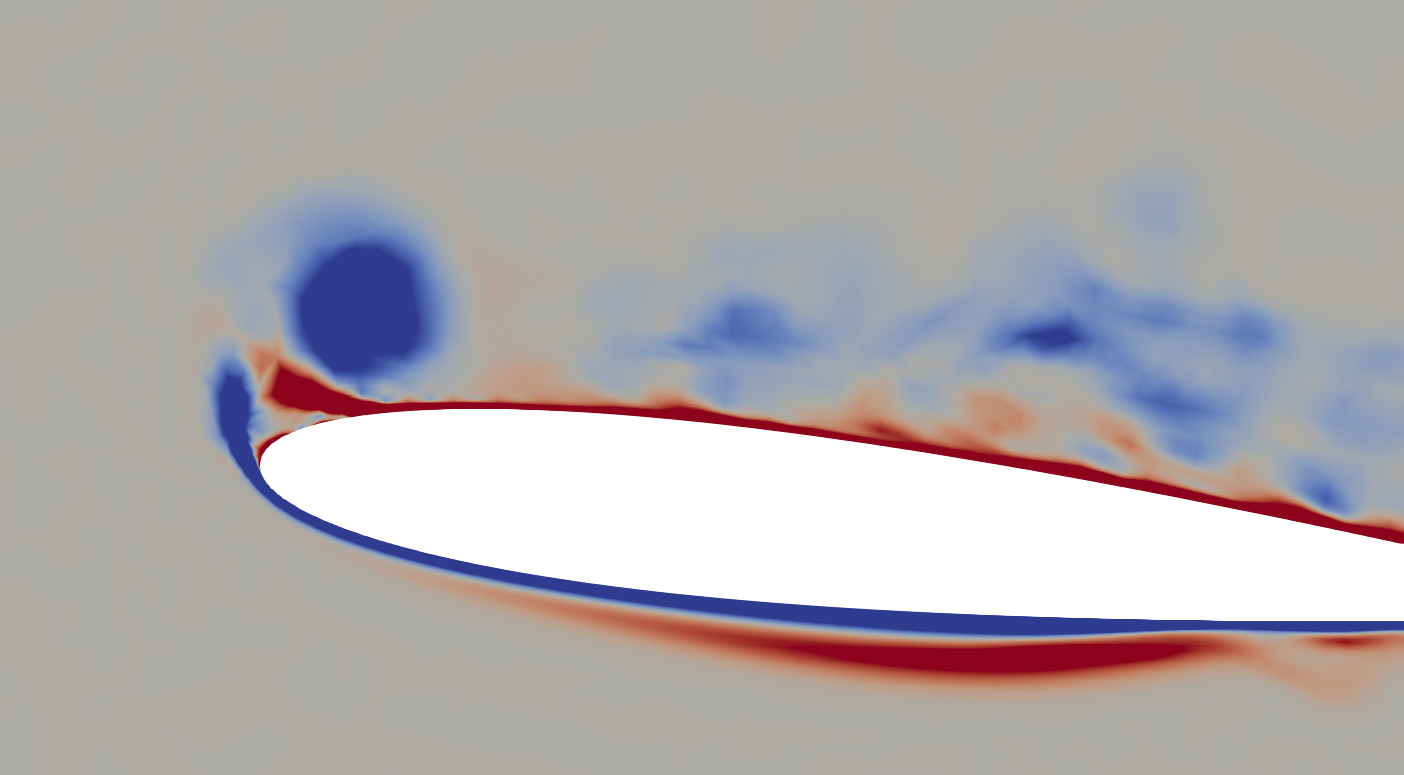
\includegraphics[width=1\textwidth]{figures/zonal_adapt_results/vorticity_plots/v2/M0/spavg/phase_240.png}
		\caption{M0\_nz25 mesh, $\psi$ = $240^\circ$}
		\label{fig:M0_sp_psi240}
		\end{subfigure}
	\end{center}
	\begin{subfigure}[b]{0.475\textwidth}
		\centering
		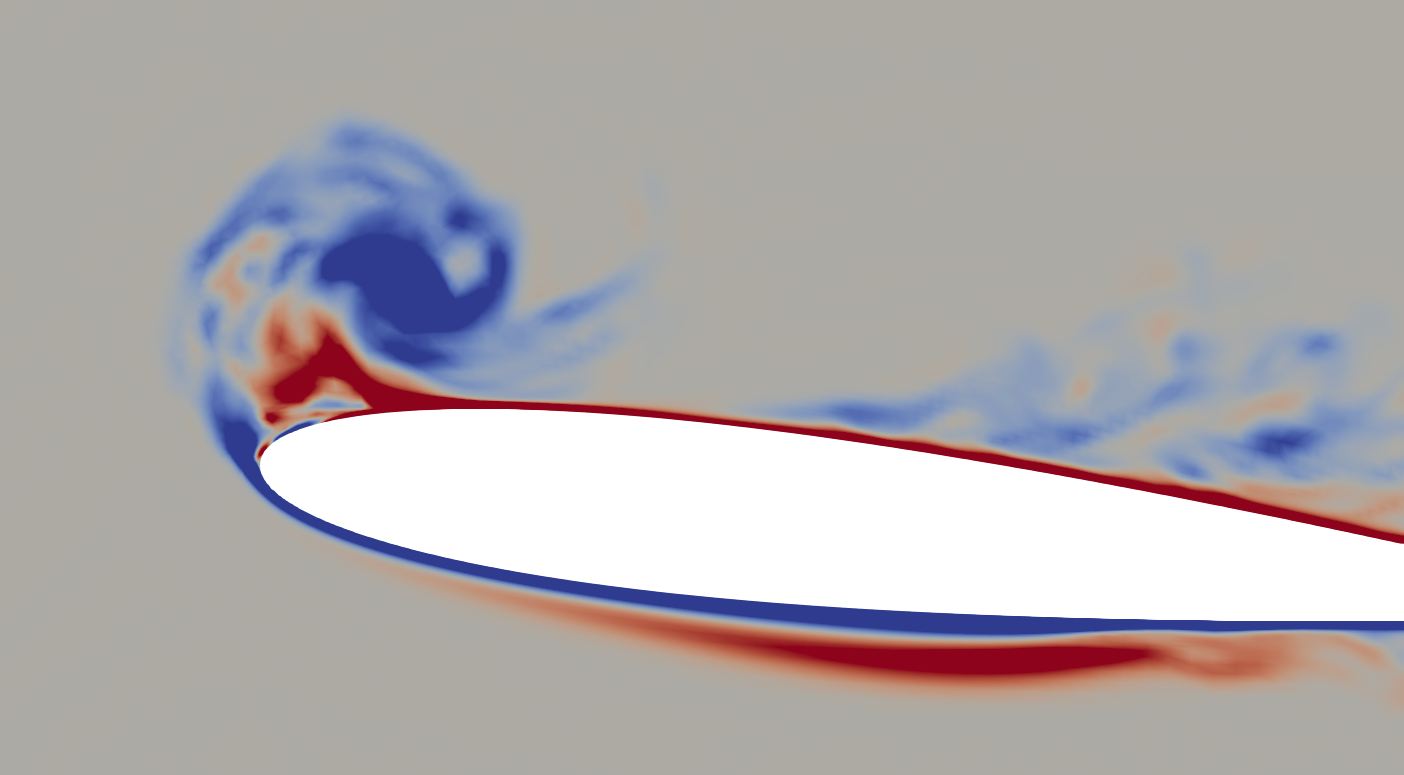
\includegraphics[width=1\textwidth]{figures/zonal_adapt_results/vorticity_plots/v2/Mza1_25/spavg/phase_240.png}
		\caption{Mza1\_nz25 mesh, $\psi$ = $240^\circ$}
		\label{fig:Mza1_25_sp_psi240}
	\end{subfigure}
	\begin{subfigure}[b]{0.475\textwidth}
	\centering
	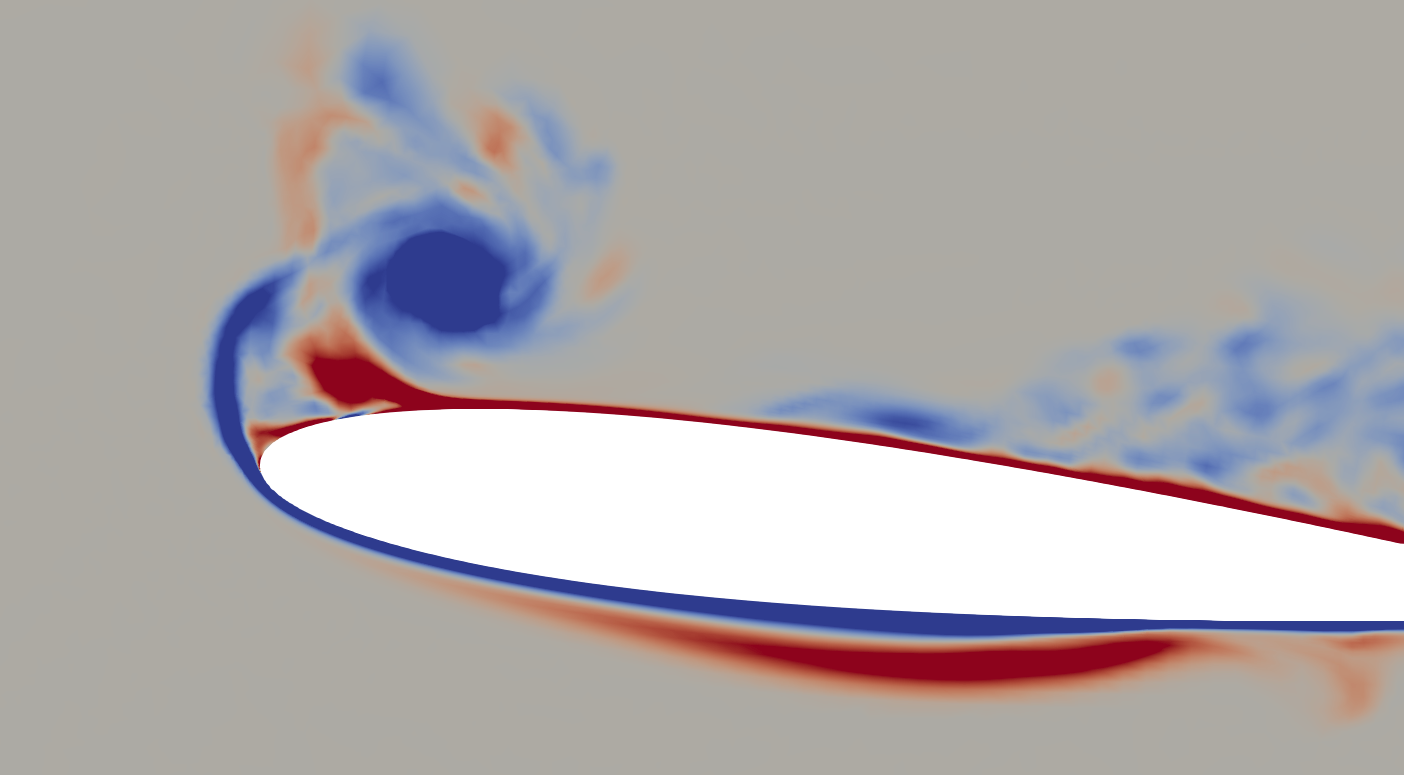
\includegraphics[width=1\textwidth]{figures/zonal_adapt_results/vorticity_plots/v2/Mza1_50/spavg/phase_240.png}
	\caption{Mza1\_nz50 mesh, $\psi$ = $240^\circ$}
	\label{fig:Mza1_50_sp_psi240}
	\end{subfigure}
	\begin{subfigure}[b]{0.475\textwidth}
		\centering
		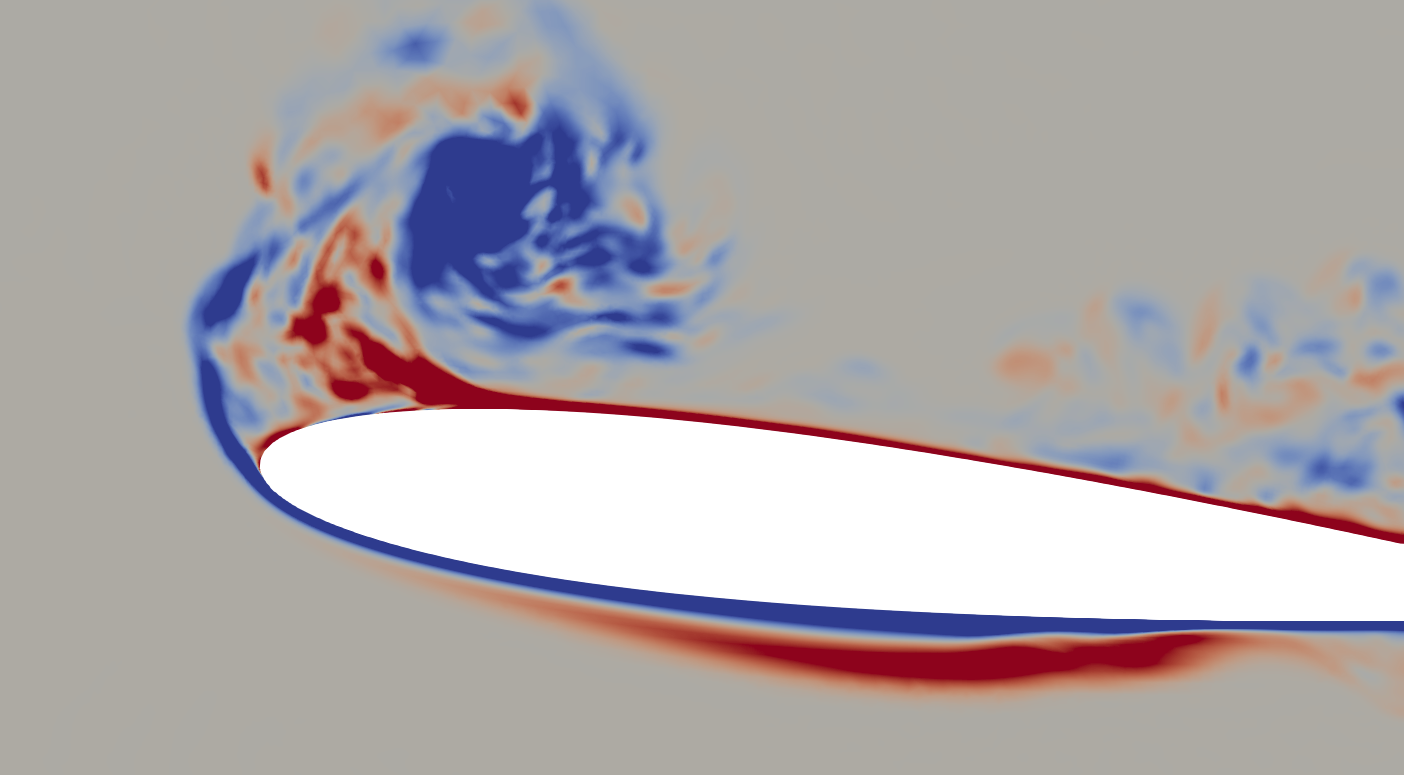
\includegraphics[width=1\textwidth]{figures/zonal_adapt_results/vorticity_plots/v2/Mza2_50/spavg/phase_240.png}
		\caption{Mza2\_nz50 mesh, $\psi$ = $240^\circ$}
		\label{fig:Mza2_50_sp_psi240}
	\end{subfigure}
%	\begin{subfigure}[b]{0.475\textwidth}
%		\centering
%		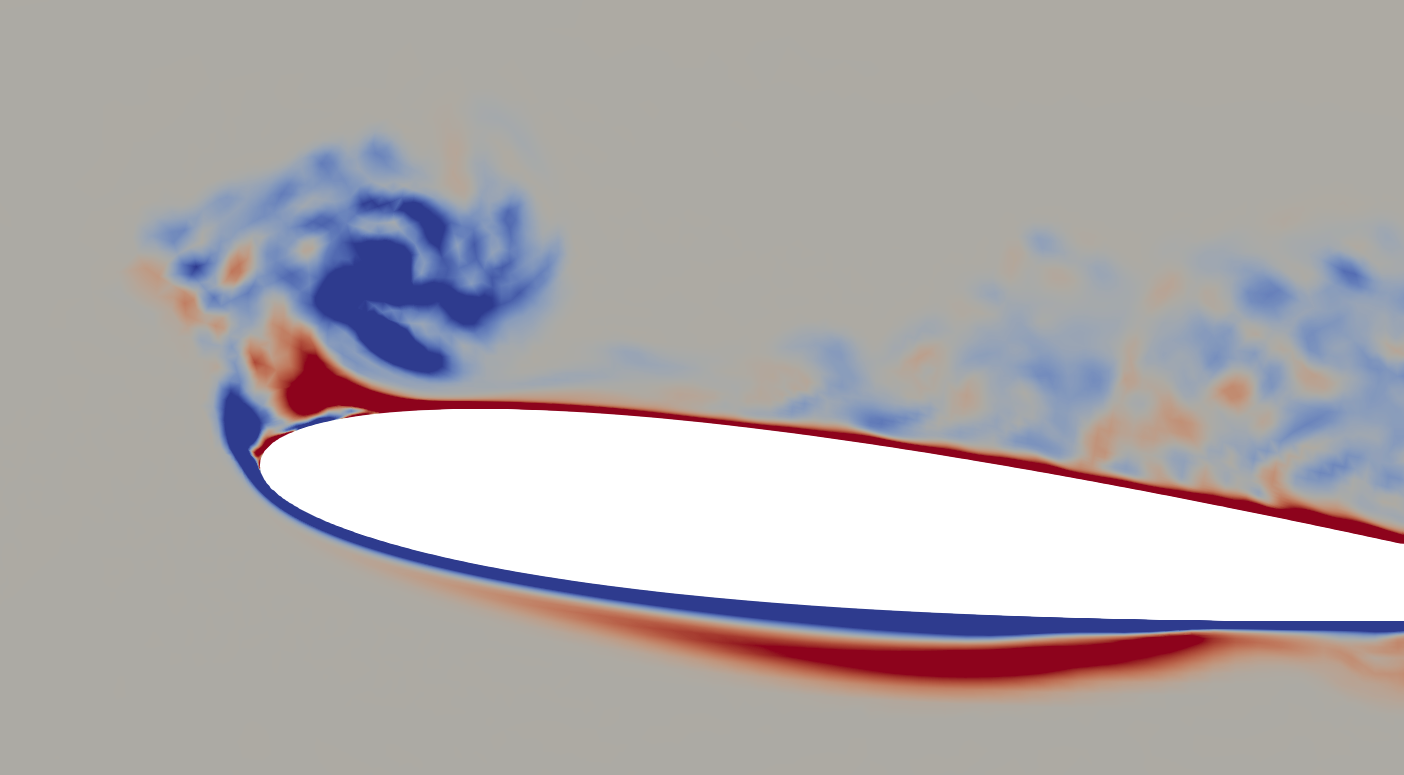
\includegraphics[width=1\textwidth]{figures/zonal_adapt_results/vorticity_plots/v2/Mza1_100/spavg/phase_240.png}
%		\caption{Mza1\_100 mesh, $\psi$ = $240^\circ$}
%		\label{fig:Mza1_100_sp_psi240}
%	\end{subfigure}
%	\begin{subfigure}[b]{0.475\textwidth}
%	\centering
%	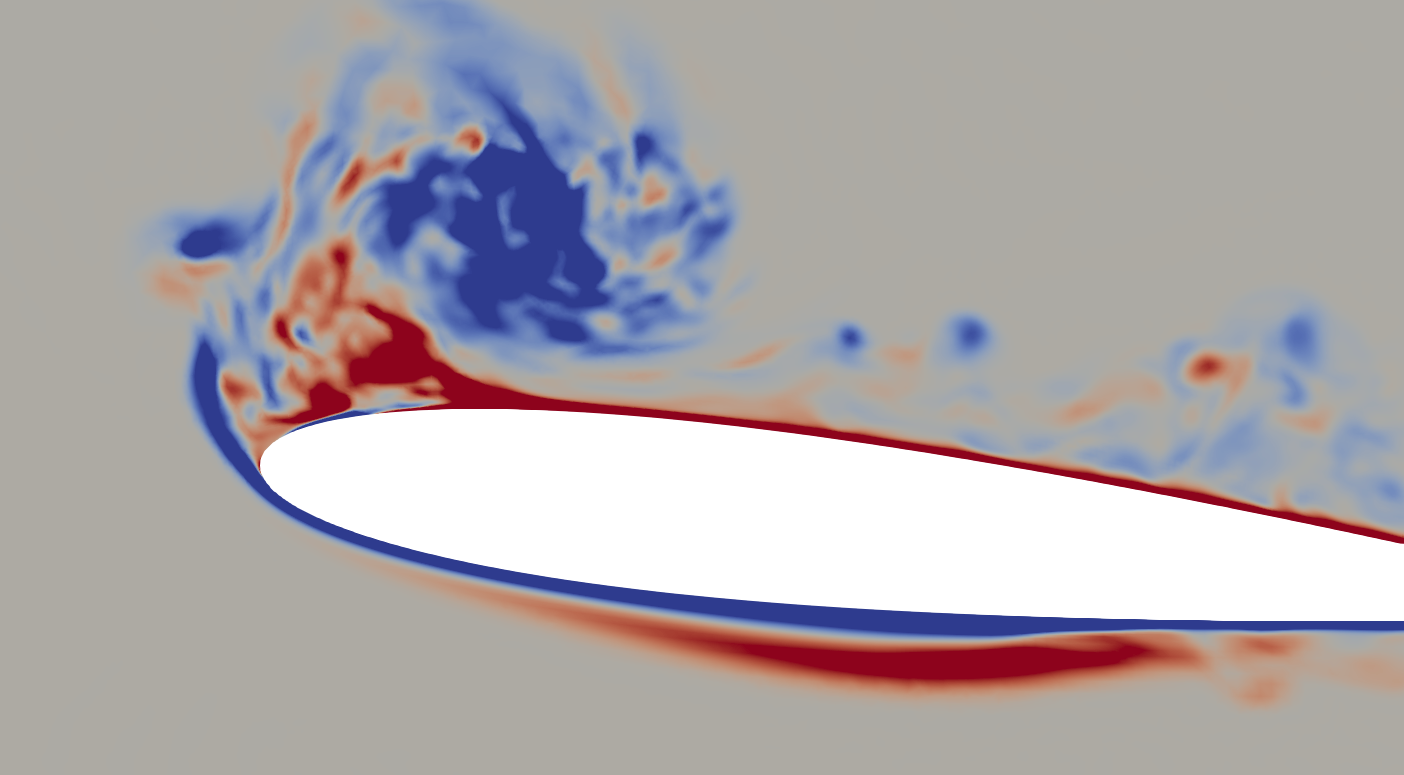
\includegraphics[width=1\textwidth]{figures/zonal_adapt_results/vorticity_plots/v2/Mza2_25/spavg/phase_240.png}
%	\caption{Mza2\_25 mesh, $\psi$ = $240^\circ$}
%	\label{fig:Mza2_25_sp_psi240}
%	\end{subfigure}	
%	\begin{subfigure}[b]{0.475\textwidth}
%		\centering
%		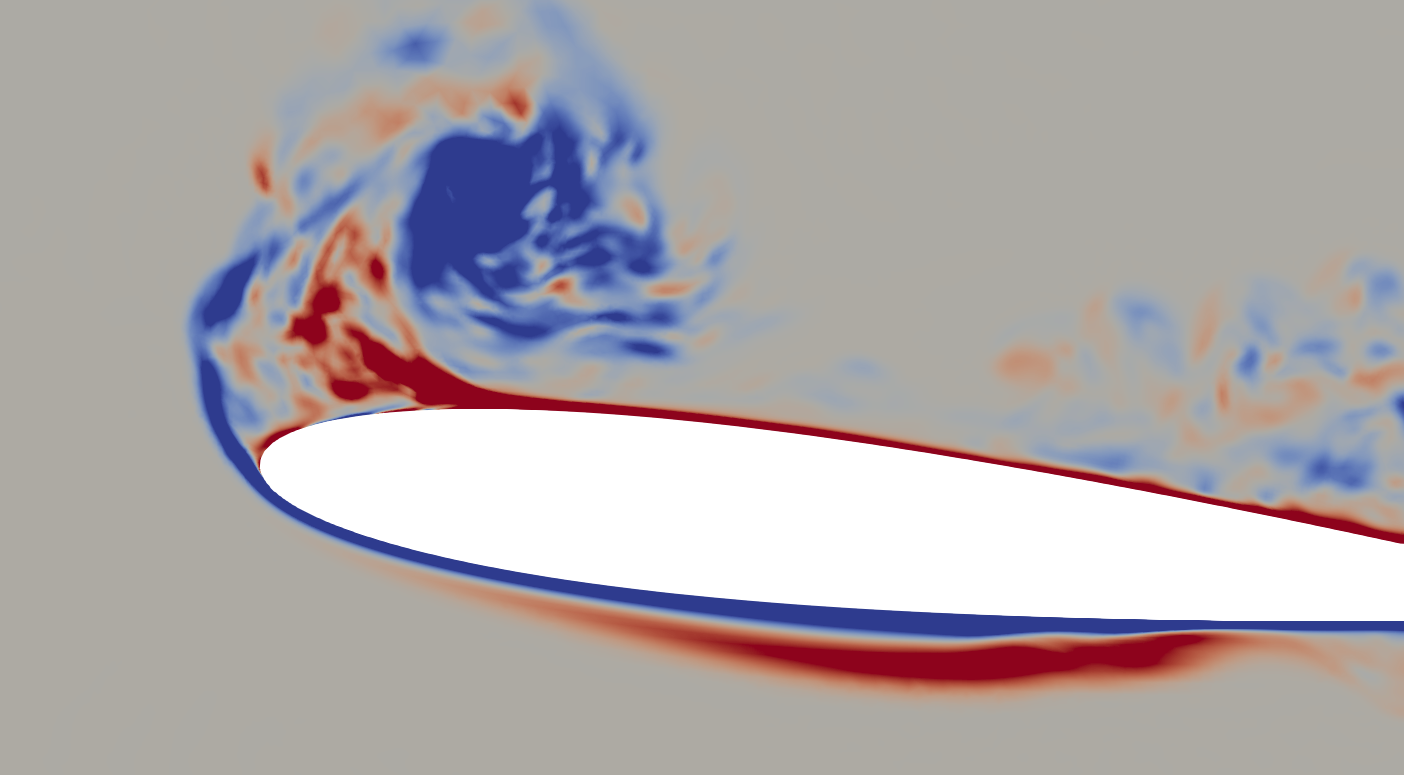
\includegraphics[width=1\textwidth]{figures/zonal_adapt_results/vorticity_plots/v2/Mza2_50/spavg/phase_240.png}
%		\caption{Mza2\_nz50 mesh, $\psi$ = $240^\circ$}
%		\label{fig:Mza2_50_sp_psi240}
%	\end{subfigure}	
	\begin{subfigure}[b]{0.475\textwidth}
		\centering
		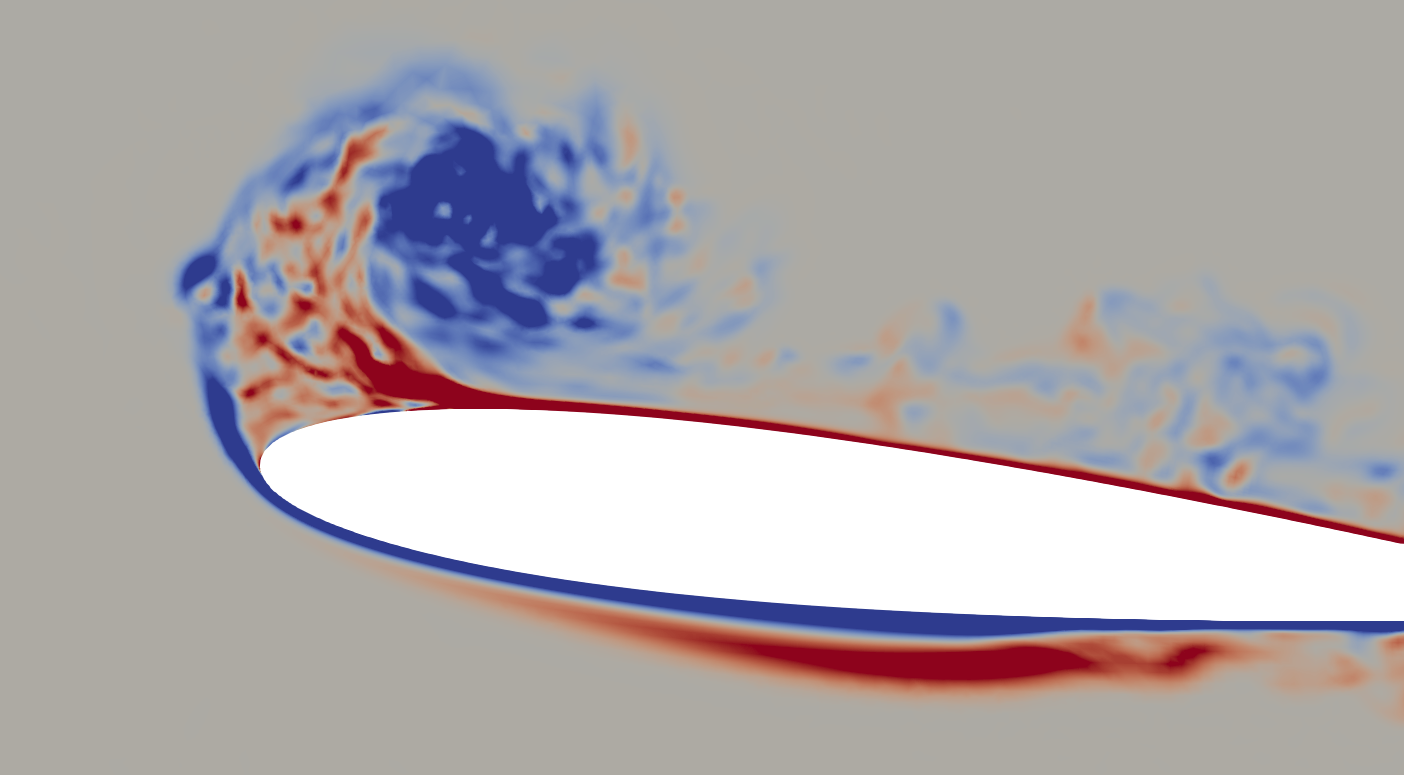
\includegraphics[width=1\textwidth]{figures/zonal_adapt_results/vorticity_plots/v2/Mza2_100/spavg/phase_240.png}
		\caption{Mza2\_nz100 mesh, $\psi$ = $240^\circ$}
		\label{fig:Mza2_100_sp_psi240}
	\end{subfigure}
	\begin{subfigure}[b]{0.475\textwidth}
	\centering
	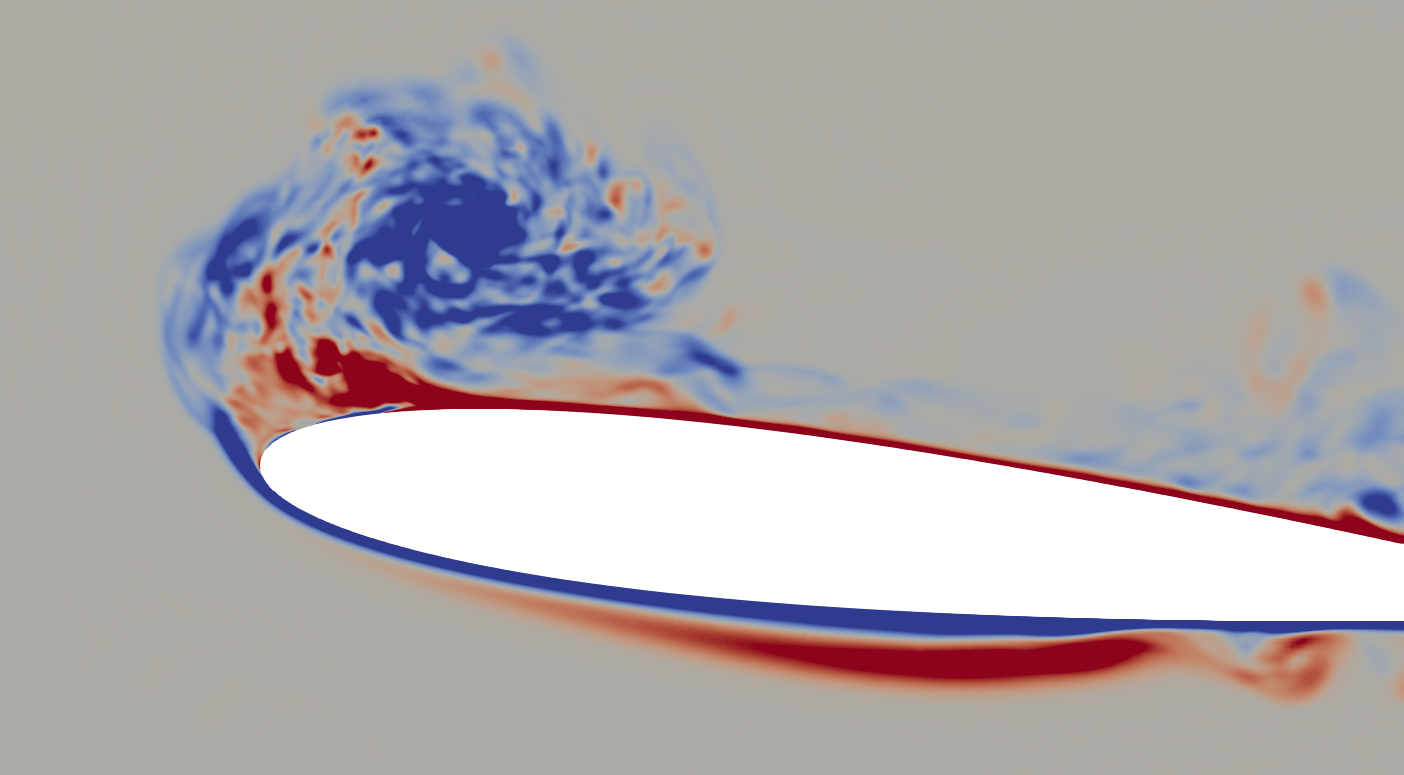
\includegraphics[width=1\textwidth]{figures/zonal_adapt_results/vorticity_plots/v2/Mza3_50/spavg/phase_240.png}
	\caption{Mza3\_nz50 mesh, $\psi$ = $240^\circ$}
	\label{fig:Mza3_50_sp_psi240}
\end{subfigure}
	\begin{subfigure}[b]{0.475\textwidth}
		\centering
		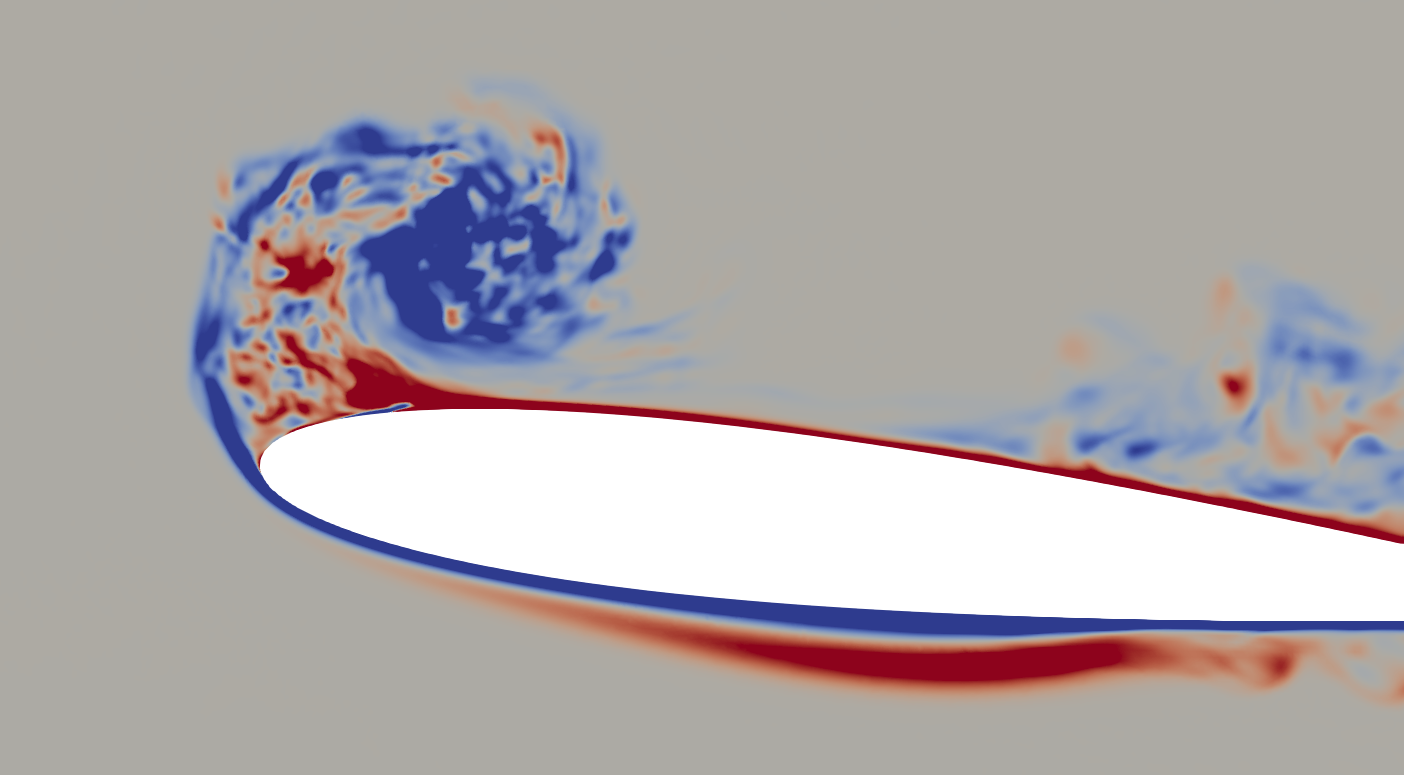
\includegraphics[width=1\textwidth]{figures/zonal_adapt_results/vorticity_plots/v2/Mza3_100/spavg/phase_240.png}
		\caption{Mza3\_nz100 mesh, $\psi$ = $240^\circ$}
		\label{fig:Mza3_100_sp_psi240}
	\end{subfigure}
	\caption{Spanwise vorticity comparison at $\psi$ = $240^\circ$ for different meshes}
	\label{fig:vorticity_zonal_240}
\end{figure}

%%=====================================
%% Phase = 270
%%=====================================


\begin{figure}[H]
	\centering
	\begin{center}
		\begin{subfigure}[b]{0.475\textwidth}
		\centering
		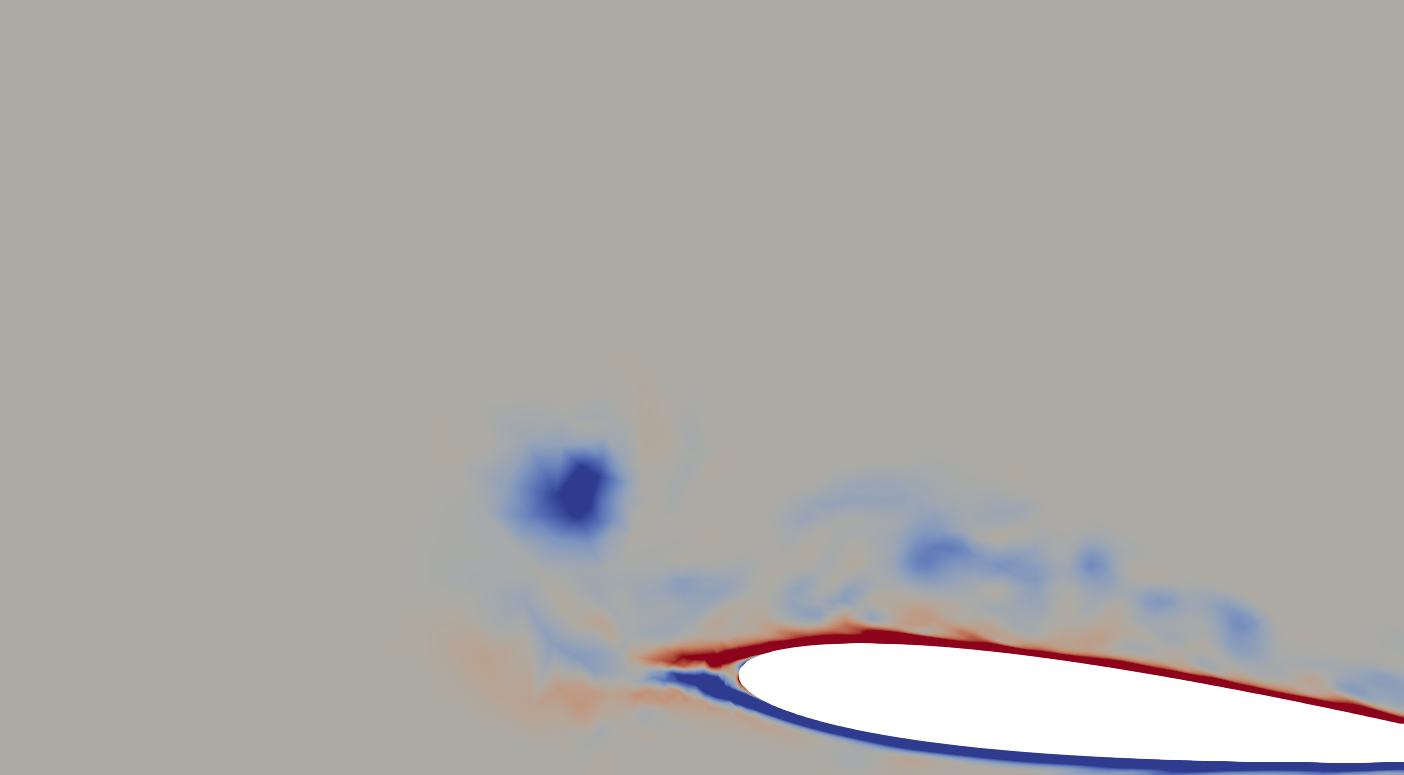
\includegraphics[width=1\textwidth]{figures/zonal_adapt_results/vorticity_plots/v3/M0/spavg/phase_270.png}
		\caption{M0\_nz25 mesh, $\psi$ = $270^\circ$}
		\label{fig:M0_sp_psi270}
		\end{subfigure}
	\end{center}
	\begin{subfigure}[b]{0.475\textwidth}
	\centering
	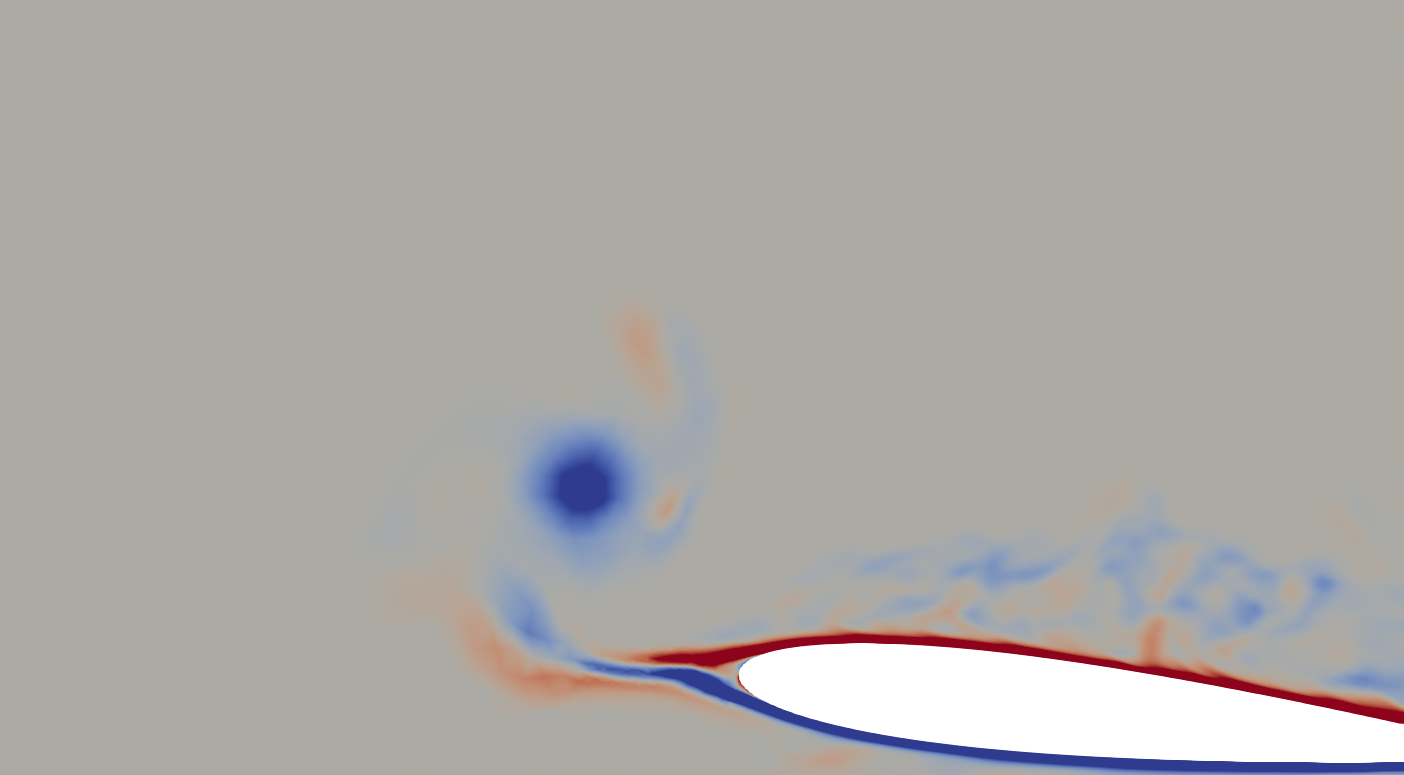
\includegraphics[width=1\textwidth]{figures/zonal_adapt_results/vorticity_plots/v3/Mza1_25/spavg/phase_270.png}
	\caption{Mza1\_nz25 mesh, $\psi$ = $270^\circ$}
	\label{fig:Mza1_25_sp_psi270}
	\end{subfigure}
	\begin{subfigure}[b]{0.475\textwidth}
		\centering
		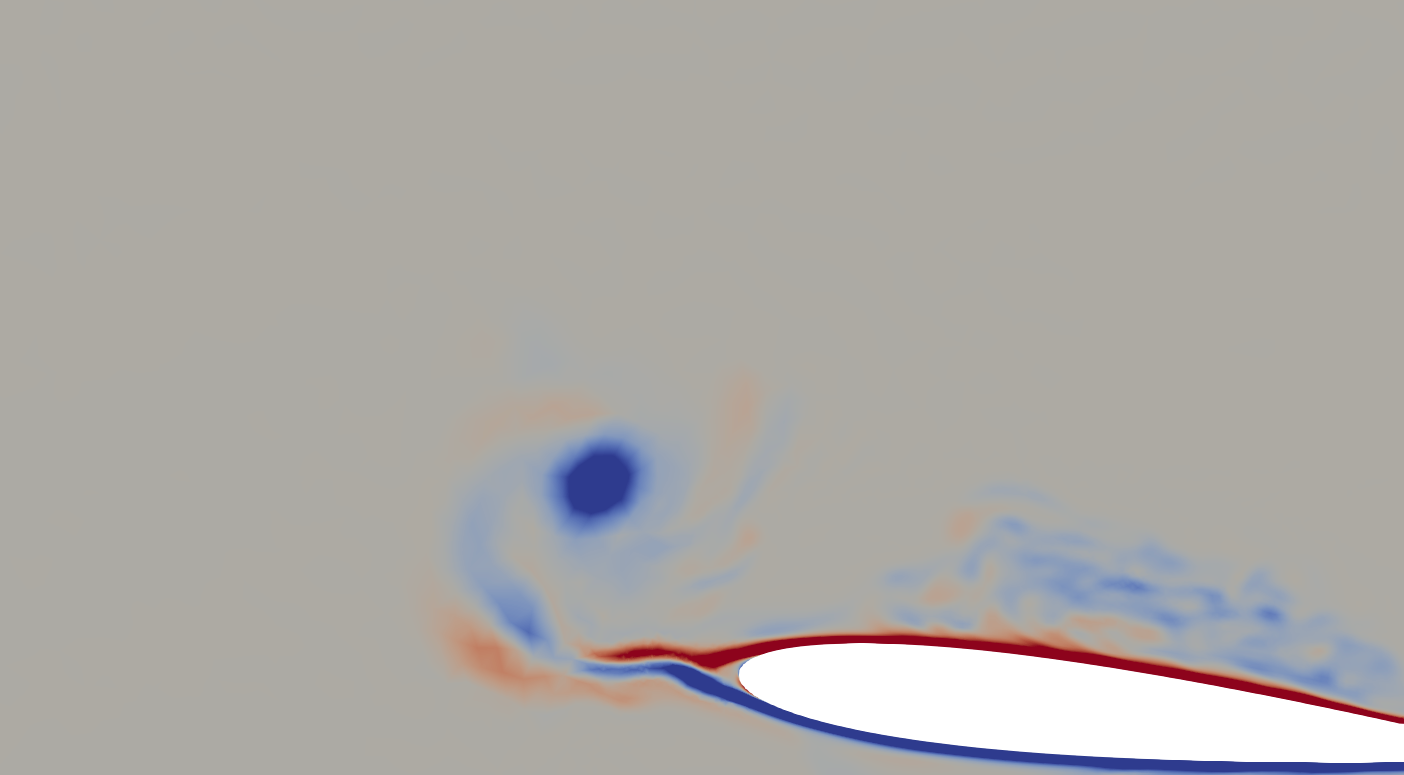
\includegraphics[width=1\textwidth]{figures/zonal_adapt_results/vorticity_plots/v3/Mza1_50/spavg/phase_270.png}
		\caption{Mza1\_nz50 mesh, $\psi$ = $270^\circ$}
		\label{fig:Mza1_50_sp_psi270}
	\end{subfigure}
%	\begin{subfigure}[b]{0.475\textwidth}
%		\centering
%		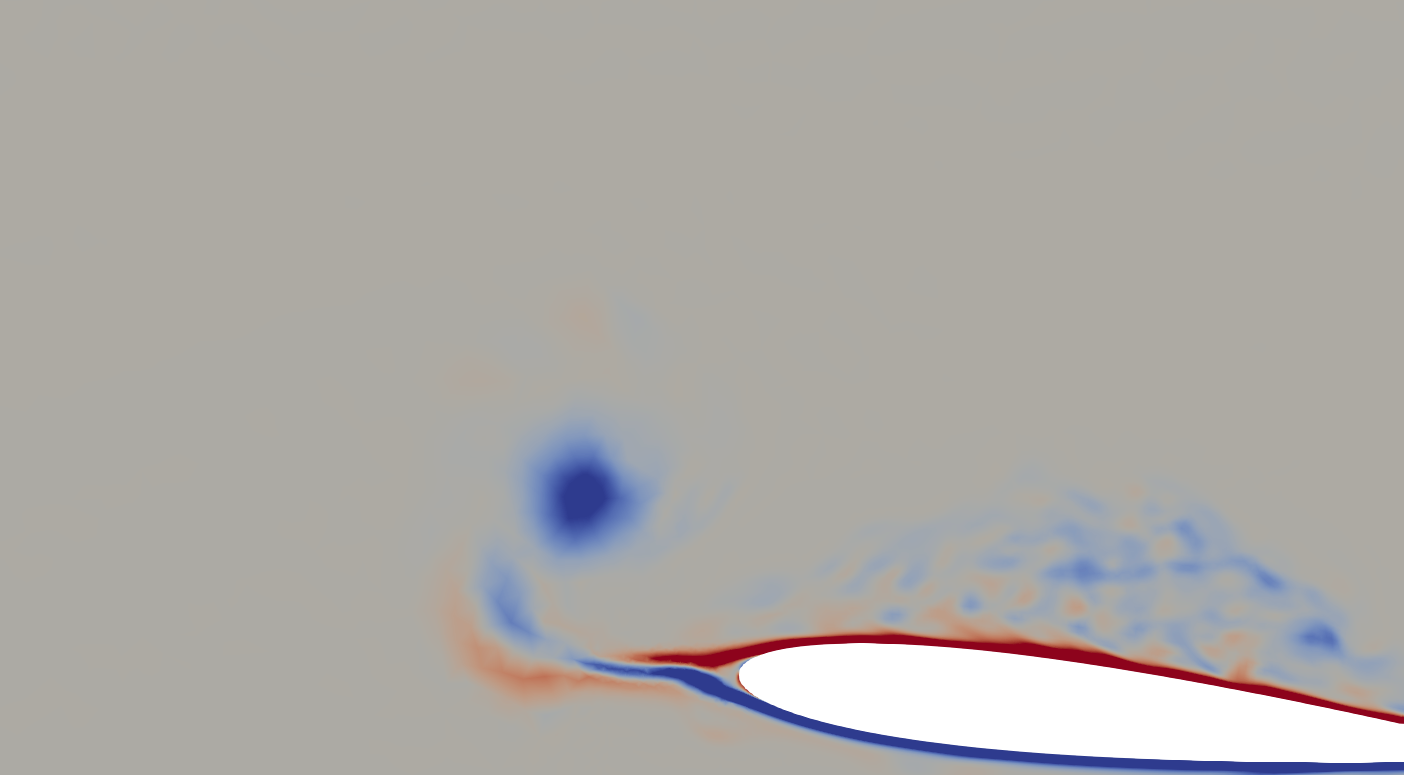
\includegraphics[width=1\textwidth]{figures/zonal_adapt_results/vorticity_plots/v3/Mza1_100/spavg/phase_270.png}
%		\caption{Mza1\_100 mesh, $\psi$ = $270^\circ$}
%		\label{fig:Mza1_100_sp_psi270}
%	\end{subfigure}
%	\begin{subfigure}[b]{0.475\textwidth}
%	\centering
%	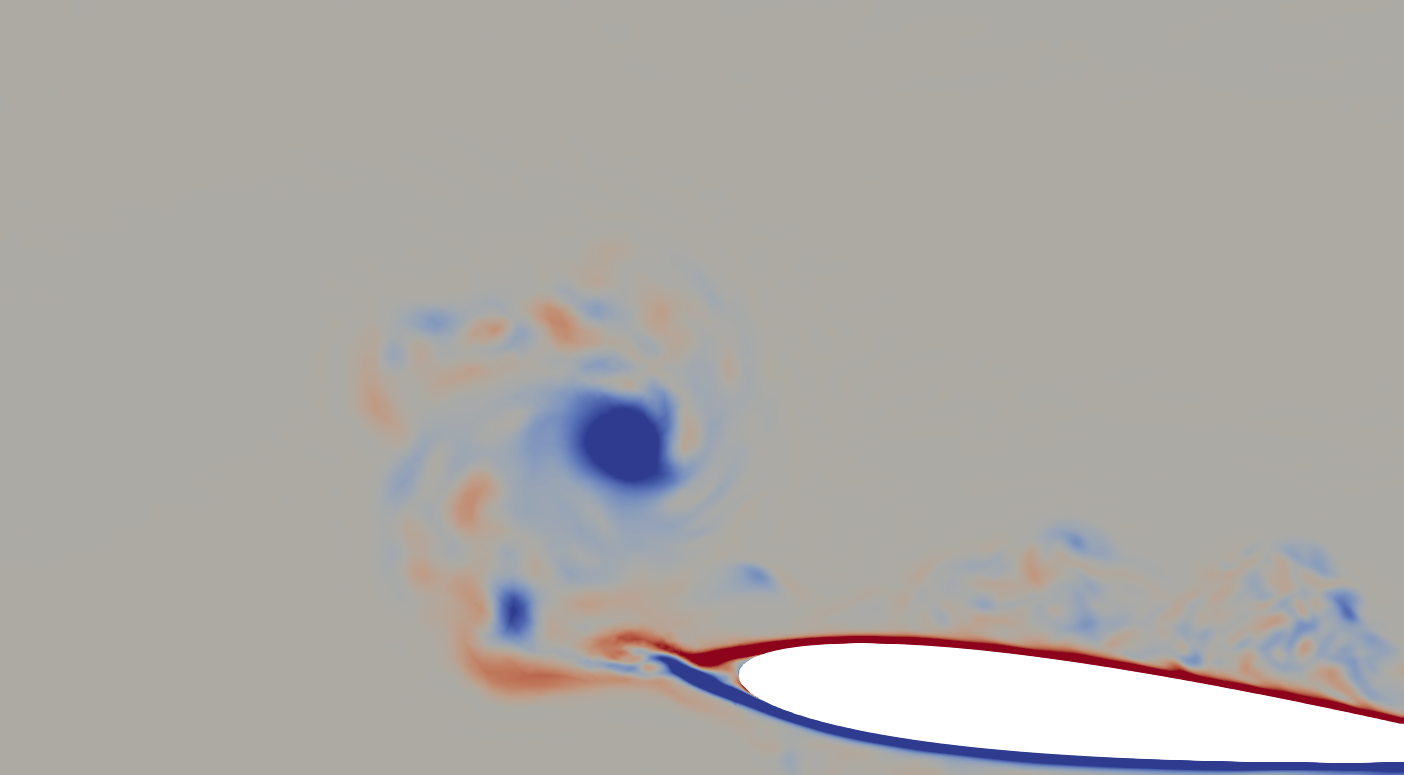
\includegraphics[width=1\textwidth]{figures/zonal_adapt_results/vorticity_plots/v3/Mza2_25/spavg/phase_270.png}
%	\caption{Mza2\_25 mesh, $\psi$ = $270^\circ$}
%	\label{fig:Mza2_25_sp_psi270}
%    \end{subfigure}	
	\begin{subfigure}[b]{0.475\textwidth}
		\centering
		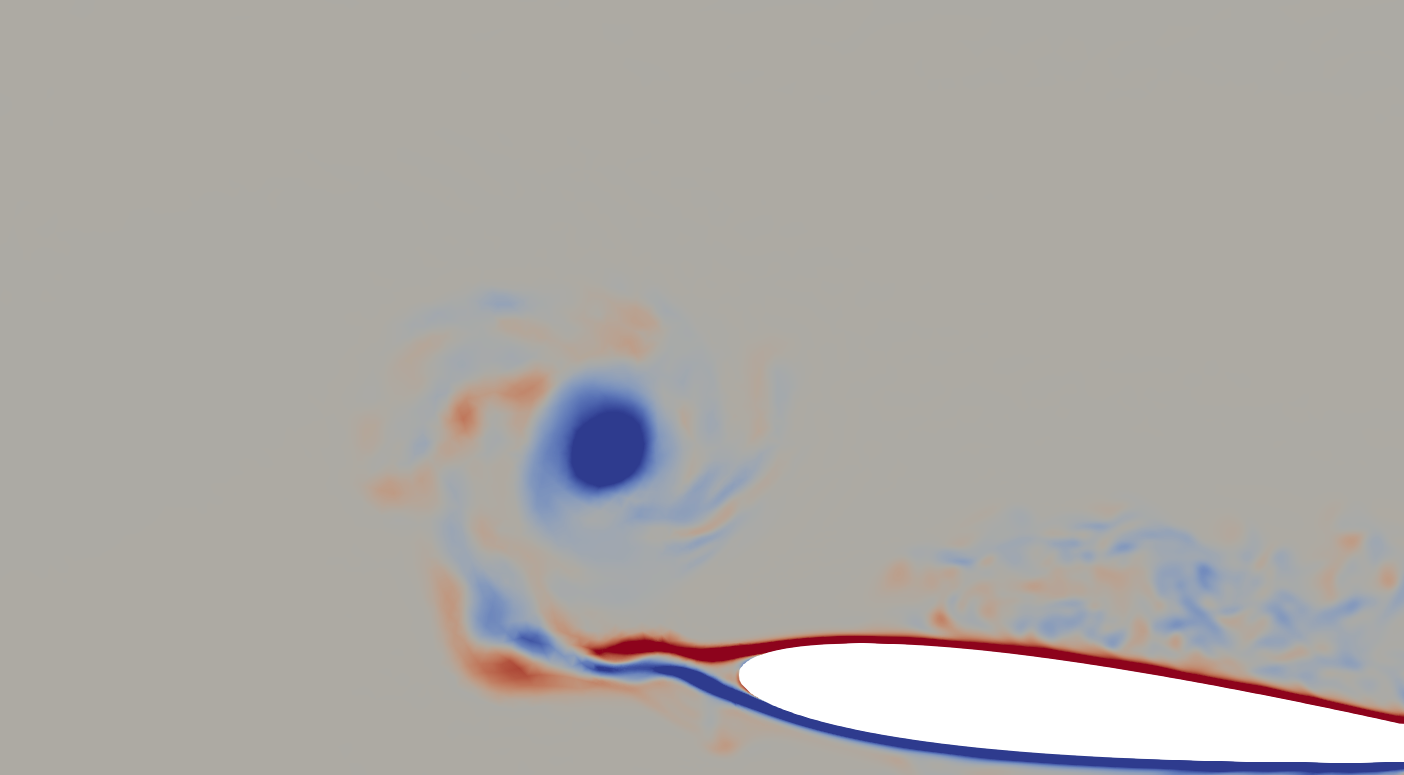
\includegraphics[width=1\textwidth]{figures/zonal_adapt_results/vorticity_plots/v3/Mza2_50/spavg/phase_270.png}
		\caption{Mza2\_nz50 mesh, $\psi$ = $270^\circ$}
		\label{fig:Mza2_50_sp_psi270}
	\end{subfigure}	
	\begin{subfigure}[b]{0.475\textwidth}
		\centering
		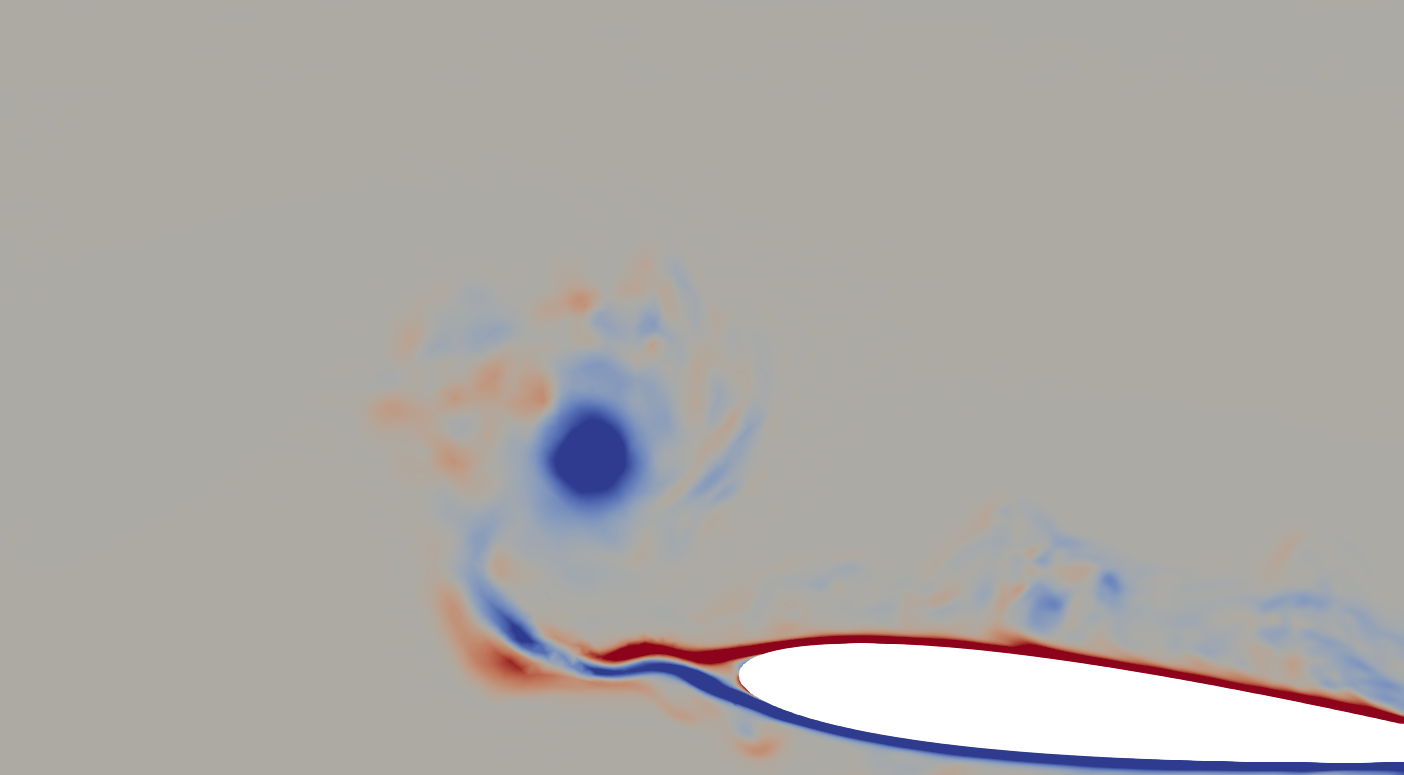
\includegraphics[width=1\textwidth]{figures/zonal_adapt_results/vorticity_plots/v3/Mza2_100/spavg/phase_270.png}
		\caption{Mza2\_nz100 mesh, $\psi$ = $270^\circ$}
		\label{fig:Mza2_100_sp_psi270}
	\end{subfigure}
	\begin{subfigure}[b]{0.475\textwidth}
	\centering
	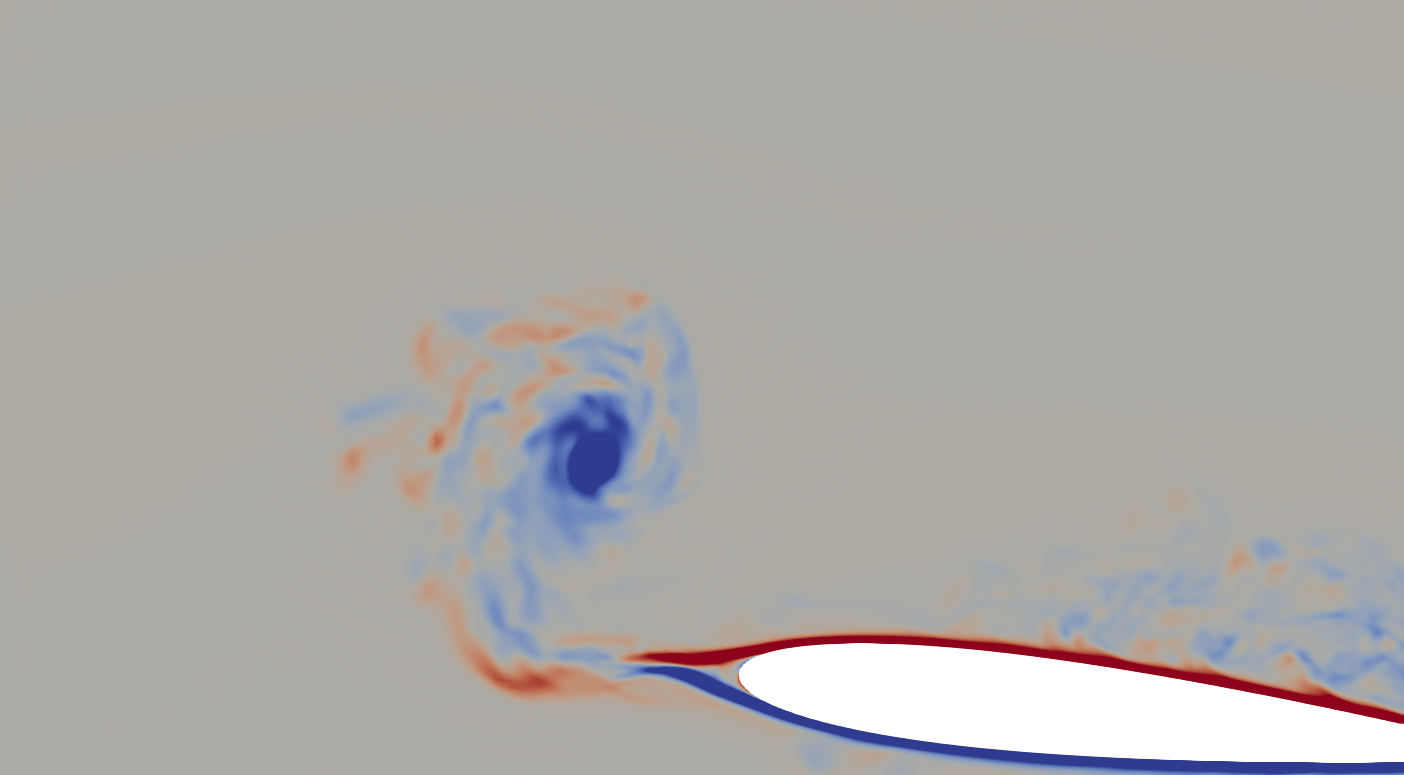
\includegraphics[width=1\textwidth]{figures/zonal_adapt_results/vorticity_plots/v3/Mza3_50/spavg/phase_270.png}
	\caption{Mza3\_nz50 mesh, $\psi$ = $270^\circ$}
	\label{fig:Mza3_50_sp_psi270}
\end{subfigure}
	\begin{subfigure}[b]{0.475\textwidth}
		\centering
		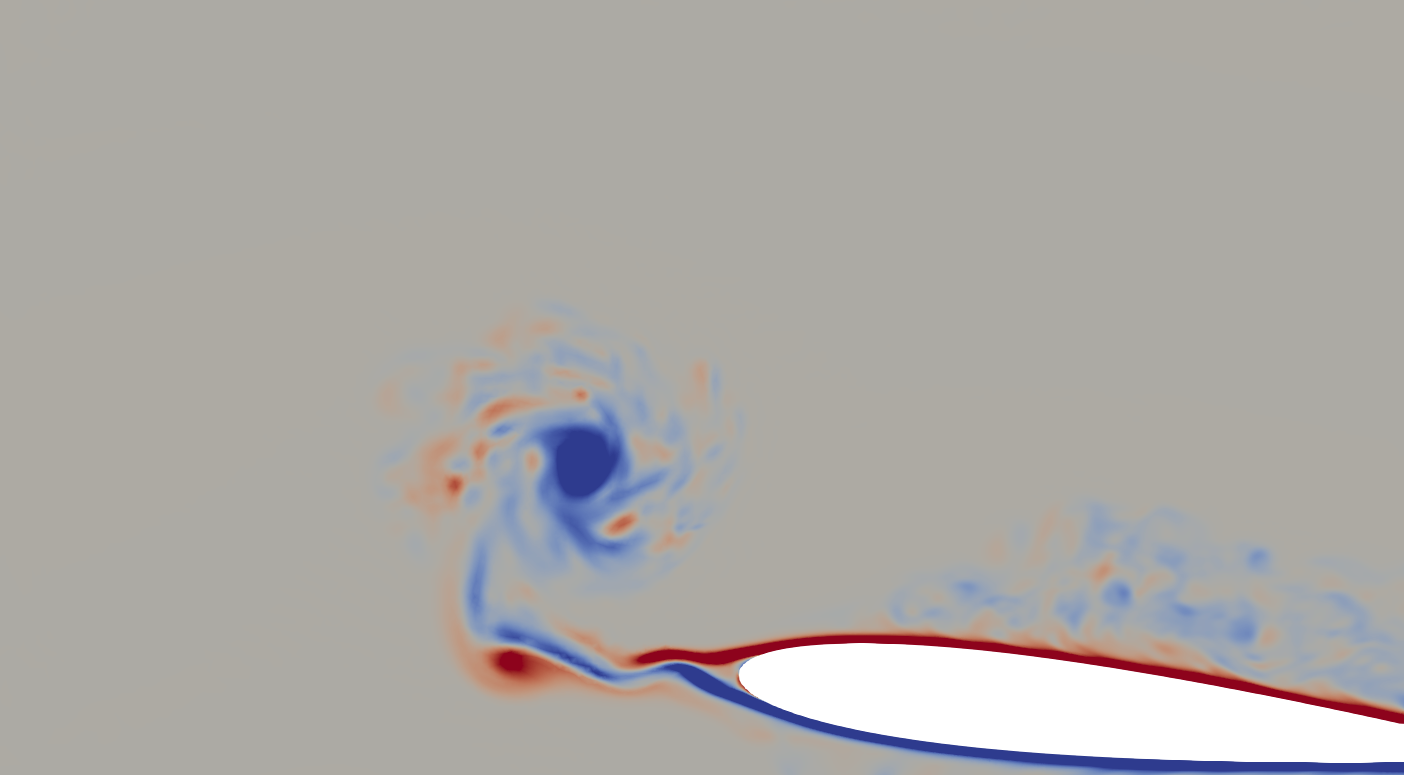
\includegraphics[width=1\textwidth]{figures/zonal_adapt_results/vorticity_plots/v3/Mza3_100/spavg/phase_270.png}
		\caption{Mza3\_nz100 mesh, $\psi$ = $270^\circ$}
		\label{fig:Mza3_100_sp_psi270}
	\end{subfigure}
	\caption{Spanwise vorticity comparison at $\psi$ = $270^\circ$ for different meshes}
	\label{fig:vorticity_zonal_270}
\end{figure}